\documentclass[11pt, oneside]{book}
\usepackage[utf8]{inputenc}
\usepackage{amsmath}
\usepackage{amssymb}
\usepackage{graphicx}
\usepackage{xcolor}
\usepackage{listings}
\usepackage{wrapfig}
\usepackage{geometry}
\usepackage{tikz}
\usepackage[greek, english]{babel}
\usetikzlibrary{positioning, decorations.pathreplacing, arrows.meta, shapes.geometric, chains, decorations.pathreplacing}
\usetikzlibrary{shapes.geometric, positioning, arrows.meta, backgrounds}
\usepackage[colorlinks=true, linkcolor=blue, urlcolor=magenta]{hyperref}

\geometry{a4paper, margin=1in}

% --- Configuration for code listings (Python) ---
\definecolor{codegreen}{rgb}{0,0.6,0}
\definecolor{codegray}{rgb}{0.5,0.5,0.5}
\definecolor{codepurple}{rgb}{0.58,0,0.82}
\definecolor{backcolour}{rgb}{0.95,0.95,0.92}

\lstdefinestyle{pythonstyle}{
    backgroundcolor=\color{backcolour},   
    commentstyle=\color{codegreen},
    keywordstyle=\color{magenta},
    numberstyle=\tiny\color{codegray},
    stringstyle=\color{codepurple},
    basicstyle=\ttfamily\footnotesize,
    breakatwhitespace=false,         
    breaklines=true,                 
    captionpos=b,                    
    keepspaces=true,                 
    numbers=left,                    
    numbersep=5pt,                  
    showspaces=false,                
    showstringspaces=false,
    showtabs=false,                  
    tabsize=2,
    language=Python
}
\lstset{style=pythonstyle}

% --- No necesitamos estos comandos si usamos el entorno titlepage ---
% \title{Concurrent Programming}
% \author{Elaborated from source document}
% \date{\today}

\begin{document}

% --- Inicio de la Portada Personalizada ---
\begin{titlepage}
    \centering
    \vspace*{2cm} % Espacio en la parte superior
    
    {\Huge\bfseries Vibenotes on Concurrent Computing\par}

    
    
    {\Large\itshape somehow by\par}
    \vspace{0.5cm}
    {\Large Andres Lopez\par}

\begin{figure}[h]
        \centering
        
\includegraphics[width=0.6\linewidth]{iimas.png}
        \label{fig:placeholder}
    \end{figure}
    
    \vspace{2.5cm} % Espacio entre título y autor
    
    \vfill % Empuja el contenido hacia arriba y abajo
    
    {\large Institute of Applied Mathematics and Systems (IIMAS)\par}
    
    \vspace{1.5cm} % Espacio sobre la fecha
    
    {\large \today\par}
    
    \vspace*{2cm} % Espacio en la parte inferior
\end{titlepage}
% --- Fin de la Portada ---

This page was unintentionally left blank, Fabian loves femboys.

\tableofcontents

\chapter{Fundamentals of Architecture and Parallel Computing}
\label{chap:fundamentos_arquitectura}

% Start of the chapter's section.
\section{Fundamental Concepts of Computer Organization and Architecture}
\label{sec:conceptos_fundamentales}

The field of computer science evolves at a dizzying speed. However, certain fundamental principles remain constant. One of the perpetual challenges is the performance barrier.

\begin{quote}
    Some algorithms are so complex that their execution on current systems would take an unreasonable amount of time, making them \textbf{computationally infeasible}. These algorithms might be feasible in the future, but history suggests that as computers become faster and more powerful, even bigger problems will arise that exceed the limits of the new technology.
\end{quote}

This race between hardware capability and problem complexity underscores the need for a deep understanding of how a computer system works. To optimize software, model complex systems, or design peripheral hardware, it is essential to know the foundations upon which modern computing is built.

\begin{itemize}
    \item \textbf{Program optimization:} It is crucial to understand how the hardware executes instructions in order to write more efficient code.
    \item \textbf{Modeling complex systems:} One must know how floating-point arithmetic, such as the \textbf{IEEE-754} standard, works both in theory and in practice to avoid precision errors.
    \begin{figure}[h!]
    \centering % Centra el diagrama en la página
    \resizebox{0.9\textwidth}{!}{% Le decimos que ocupe el 90% del ancho del texto
        % --- TU CÓDIGO TIKZ ORIGINAL VA AQUÍ DENTRO ---
        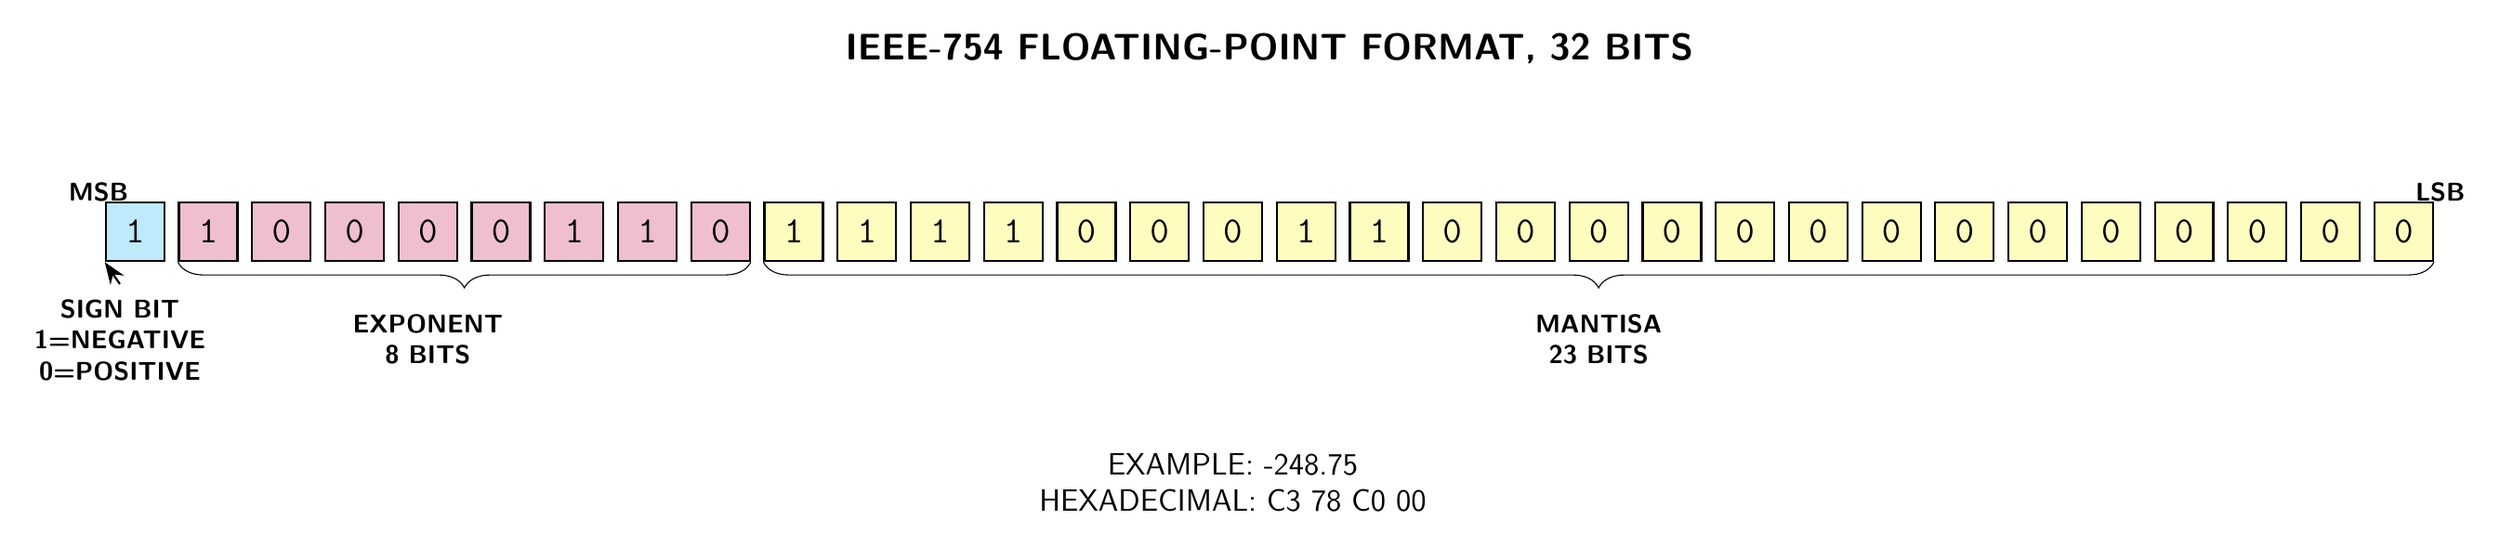
\begin{tikzpicture}[
            % --- Styles for the nodes ---
            bit/.style={
                draw, thick, rectangle, minimum size=0.8cm, font=\Large\ttfamily
            },
            sign/.style={bit, fill=cyan!25},
            exponent/.style={bit, fill=purple!25},
            mantissa/.style={bit, fill=yellow!25},
            title/.style={font=\Large\bfseries\sffamily},
            label_style/.style={font=\sffamily\bfseries, align=center}
        ]

        % --- Diagram Title ---
        \node[title] at (16.5, 2.5) {IEEE-754 FLOATING-POINT FORMAT, 32 BITS};

        % --- MSB and LSB Labels ---
        \node[label_style, above=0.3cm of {(0.5,0)}] {MSB};
        \node[label_style, above=0.3cm of {(32.5,0)}] {LSB};

        % --- Draw the 32 bits using a loop ---
        \foreach \valor [count=\i from 1] in {1,1,0,0,0,0,1,1,0,1,1,1,1,0,0,0,1,1,0,0,0,0,0,0,0,0,0,0,0,0,0,0} {
            \ifnum\i=1
                \node[sign] (bit\i) at (\i, 0) {\valor};
            \else
                \ifnum\i<10
                    \node[exponent] (bit\i) at (\i, 0) {\valor};
                \else
                    \node[mantissa] (bit\i) at (\i, 0) {\valor};
                \fi
            \fi
        }

        % --- Brace and label for the Exponent ---
        \draw[decorate, decoration={brace, amplitude=10pt, mirror}] 
            (bit2.south west) -- (bit9.south east);
        \node[label_style, below=0.6cm of bit5.south] {EXPONENT \\ 8 BITS};

        % --- Brace and label for the Mantissa ---
        \draw[decorate, decoration={brace, amplitude=10pt, mirror}] 
            (bit10.south west) -- (bit32.south east);
        \node[label_style, below=0.6cm of bit21.south] {MANTISA \\ 23 BITS};

        % --- Arrow and label for the Sign Bit ---
        \node[label_style, below left=0.4cm and -1.5cm of bit1] (signtext) {SIGN BIT \\ 1=NEGATIVE \\ 0=POSITIVE};
        \draw[-{Stealth[length=3mm]}, thick] (signtext.north) ++(0, 0.1) -- (bit1.south west);

        % --- Example Information ---
        \node[label_style, font=\sffamily\large, below=2.5cm of bit16.south] 
            {EXAMPLE: -248.75 \\ HEXADECIMAL: C3 78 C0 00};

        \end{tikzpicture}
    }% Fin del \resizebox
    \caption{Diagram of the 32-bit IEEE-754 floating-point format.}
    \label{fig:ieee754_format}
\end{figure}
    \item \textbf{Peripheral design:} The development of hardware or the software that controls it (drivers) demands a detailed knowledge of Input/Output (I/O) mechanisms.
    \item \textbf{Embedded systems:} When working with limited resources (memory, computing power), it is vital to know the architecture to maximize efficiency.
    \item \textbf{Benchmarking:} One must be familiar with the methods for measuring and comparing the performance of different systems fairly and accurately.
\end{itemize}

These points demonstrate a symbiotic and inescapable relationship between hardware and software. Below, the two key concepts that define this relationship are broken down: computer architecture and organization.

\subsection{Computer Architecture}
Computer architecture refers to the attributes of a system that are visible to a programmer. That is, those aspects that have a direct impact on the logical execution of a program. It focuses on the \textbf{structure and behavior} of the system from an abstract perspective.

\begin{itemize}
    \item \textbf{Main attributes:} It includes the instruction set architecture (ISA), data types, the number and type of registers, addressing modes, main memory access methods, and I/O mechanisms.
    \item \textbf{Focus:} It answers the question: \textit{How do I design a computer?} 
    \item \textbf{Formal definition:} It is the combination of its hardware components (specifically microprocessors) plus its \textbf{Instruction Set Architecture (ISA)}. The ISA acts as the crucial interface between the software and the hardware, allowing the programmer to "talk" to the machine.
\end{itemize}

\subsection{Computer Organization}
Computer organization deals with the physical implementation of the architecture. It addresses how the hardware components are interconnected and operate to realize the architectural specifications. These details are often transparent to the programmer.

\begin{itemize}
    \item \textbf{Main attributes:} It encompasses control signals, interfaces between components, memory technology, and signaling methods. That is, all the physical aspects of the system.
    \item \textbf{Focus:} It answers the question: \textit{How does a computer work?}
    \item \textbf{Relationship with architecture:} The implementation of an architecture is known as its organization. Frequently, the organization is also referred to as \textbf{microarchitecture}.
\end{itemize}

\subsubsection{Key Differences Between Organization and Architecture}

\begin{figure}[h!]
    \centering
    \begin{tikzpicture}[
        % Estilos globales para nodos y líneas
        level/.style={ellipse, draw=green!50!black, fill=green!10!white, thick, align=center, minimum width=3.5cm, minimum height=0.9cm, font=\sffamily\bfseries\color{green!40!black}},
        arrow/.style={-Stealth, thick, black},
        label_side/.style={font=\sffamily\bfseries\color{green!50!black}, align=left},
        label_bottom/.style={font=\sffamily\bfseries\color{blue!70!black}},
        line_label/.style={font=\sffamily\bfseries\color{green!50!black}, rotate=90, anchor=south},
        vline/.style={-{Bar[width=4pt]}-{Bar[width=4pt]}, thick, draw=green!50!black},
        background rectangle/.style={fill=blue!5!white, draw=black, line width=2pt},
        show background fill,
        show background draw
    ]

    % --- Nodos para los "nivaveles" ---
    \node[level] (app_program) at (0,0) {Application Program};
    \node[level, below=0.5cm of app_program] (app_design) {Application Design};
    \node[level, below=0.5cm of app_design] (sys_design) {System Design};
    \node[level, below=0.5cm of sys_design] (comp_design) {Computer Design};
    \node[level, below=0.5cm of comp_design] (logic_design) {Logic Design};
    \node[level, below=0.5cm of logic_design] (circ_design) {Circuit Design};
    \node[level, below=0.5cm of circ_design] (comp_component) {Computer Component};

    % --- Flechas de conexión ---
    \foreach \source/\target in {app_program/app_design, app_design/sys_design, sys_design/comp_design, comp_design/logic_design, logic_design/circ_design, comp_design/comp_component} {
        \draw[arrow] (\source) -- (\target);
    }

    % --- Etiquetas laterales y verticales ---
    \node[label_side, left=2.8cm of app_program.west] {High Level};
    \node[label_side, left=2.8cm of comp_component.west] {Low Level};

    % Se define una coordenada X a la derecha y se dibuja una línea vertical
    \coordinate (linea_derecha) at ([xshift=2.2cm]app_program.east);
    \draw[vline] (linea_derecha |- app_program.center) -- (linea_derecha |- sys_design.center) node[midway, line_label] {Software};
    \draw[vline] (linea_derecha |- comp_design.center) -- (linea_derecha |- comp_component.center) node[midway, line_label] {Hardware};

    % Se define una coordenada X a la izquierda y se dibuja una línea vertical
    \coordinate (linea_izquierda) at ([xshift=-2.2cm]app_program.west);
    \draw[vline] (linea_izquierda |- sys_design.center) -- (linea_izquierda |- comp_design.center) node[midway, line_label] {C. Architecture};
    \draw[vline] (linea_izquierda |- logic_design.center) -- (linea_izquierda |- circ_design.center) node[midway, line_label] {C. Organization $|$};
    
    % --- Etiqueta inferior ---
    \node[label_bottom, below=1cm of comp_component] {Computer System};

    \end{tikzpicture}
    \caption{Computer System Levels of Abstraction (don't even try to understand this, it's pointless)}
    \label{fig:computer_levels}
\end{figure}

To solidify the distinction, the table \ref{tab:arq_vs_org} summarizes the fundamental differences.

\begin{table}[h!]
    \centering
    \caption{Computer Architecture vs. Organization}
    \label{tab:arq_vs_org}
    \begin{tabular}{|p{0.45\textwidth}|p{0.45\textwidth}|}
        \hline
        \textbf{Computer Architecture} & \textbf{Computer Organization} \\
        \hline
        Describes \textbf{what} the computer does. & Describes \textbf{how} it does it. \\
        \hline
        Deals with the \textbf{functional} and logical behavior. & Deals with the \textbf{structural} and physical relationship. \\
        \hline
        \textbf{High-level} design issues (visible to the programmer). & \textbf{Low-level} design issues (transparent to the programmer). \\
        \hline
        Defines the instruction set (ISA). & Indicates performance (FLOPS, Gbps). \\
        \hline
        To design a computer, its architecture is defined first. & The organization is chosen and designed based on the defined architecture. \\
        \hline
        Also known as \textbf{ISA (Instruction Set Architecture)}. & Frequently referred to as \textbf{microarchitecture}. \\
        \hline
        Comprises logical attributes: ISA, registers, data types, addressing modes. & Consists of physical units: circuit designs, peripherals, adders. \\
        \hline
        \textbf{Examples of architectures:} x86 (Intel, AMD), ARM, SPARC, PowerPC. & \textbf{Examples of organization:} Specific implementations like Intel Core i9 vs AMD Ryzen 9 (both x86), or Apple M3 (ARM). \\
        \hline
    \end{tabular}
\end{table}

\paragraph{Illustrative Example:}
An \textbf{architectural} decision is whether a computer will have a multiplication instruction in its ISA. Once it is decided that it will, an \textbf{organizational} decision is whether that instruction will be implemented by a specialized hardware multiplication unit or by an algorithm that iteratively uses the system's addition unit. The organizational decision will be based on factors such as cost, physical space, power consumption, and desired speed.

\subsection{Hardware-Software Equivalence Principle}
Modern computers are, in essence, implementations of algorithms that execute other algorithms. This leads to a fundamental concept:

\begin{quote}
    \textbf{Principle of Hardware and Software Equivalence:} Any task performed by software can also be performed by hardware, and any operation performed directly by hardware can be simulated by software.
\end{quote}

The choice between a hardware or software implementation for a specific task depends on criteria such as speed, cost, flexibility, and production volume.

\begin{itemize}
    \item \textbf{Hypervisors:} They are a clear example. A \textit{Bare-metal (type 1)} hypervisor runs directly on the hardware, acting almost like a virtual hardware layer. A \textit{Hosted (type 2)} hypervisor runs on top of an operating system, behaving more like a traditional software application.
    \item \textbf{FPGAs (Field Programmable Gate Arrays):} They are the epitome of this principle. An FPGA is an integrated circuit that can be configured by the user to emulate any digital circuit. It allows "designing" hardware through software (using hardware description languages like VHDL or Verilog). An FPGA is composed of:
    \begin{itemize}
        \item \textbf{CLBs (Configurable Logic Blocks):} They are the computing elements. Each CLB typically contains:
        \begin{itemize}
            \item \textbf{LUT (Look-Up Table):} A small memory that can implement any logical function.
            \item \textbf{D-type Flip-flop:} Acts as a one-bit memory to store the result of the LUT.
            \item \textbf{MUX (Multiplexers):} Select and route signals.
        \end{itemize}
        \item \textbf{Interconnects and Switching Matrices:} They allow connecting the CLBs to each other.
        \item \textbf{I/O Blocks:} They connect the FPGA to the outside world.
    \end{itemize}
\end{itemize}
FPGAs are widely used in communications, AI, the automotive industry, and aerospace due to their ability to create custom, high-performance hardware solutions.

\subsection{The Essential Components of a Computer System}
\label{subsec:essential_components}

At its core, any functional computer system is built from three fundamental types of hardware components:

\begin{figure}[h]
    \centering
    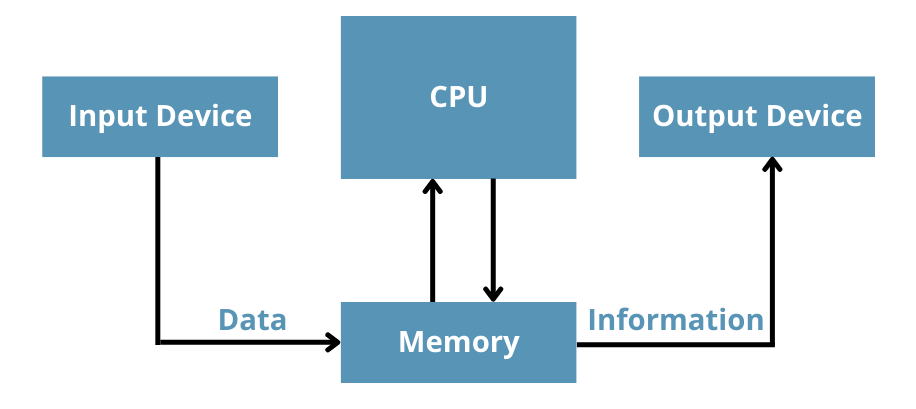
\includegraphics[width=0.5\linewidth]{CPU IO Memory.png}
    \label{fig:placeholder}
\end{figure}

\begin{enumerate}
    \item A \textbf{processor (CPU)} to interpret and execute programs.
    \item A \textbf{memory} to store both data and programs.
    \item A \textbf{mechanism} to transfer data to and from the outside world (Input/Output or I/O).
\end{enumerate}
These components work in concert, forming the foundation upon which all software runs.

\subsubsection{The Central Processing Unit (CPU)}
The Central Processing Unit (CPU) is the principal hardware component that performs the actual computation. It consists of three main parts:
\begin{description}
    \item[Arithmetic Logic Unit (ALU)] This is the digital calculator of the CPU. It performs arithmetic calculations (e.g., addition, subtraction) and logical operations (e.g., AND, OR, NOT).
    \item[Control Unit (CU)] The CU acts as the system's director. It fetches instructions from memory and directs the flow of data, ensuring it arrives at the correct locations within the system at the appropriate time.
    \item[Registers] These are very small, extremely fast storage locations built directly into the processor die. They hold data that the CPU needs to access almost instantly, such as the current instruction being executed or the result of an ALU calculation.
\end{description}

\subsubsection{Memory}
Memory is where a computer stores the instructions and data it needs to operate. It is not a single entity but rather a \textbf{hierarchy} of different levels, designed to provide the best possible performance at the lowest cost. This hierarchy ranges from very fast, small, and expensive memory to very slow, large, and cheap memory.

\begin{figure}[h!]
    \centering
    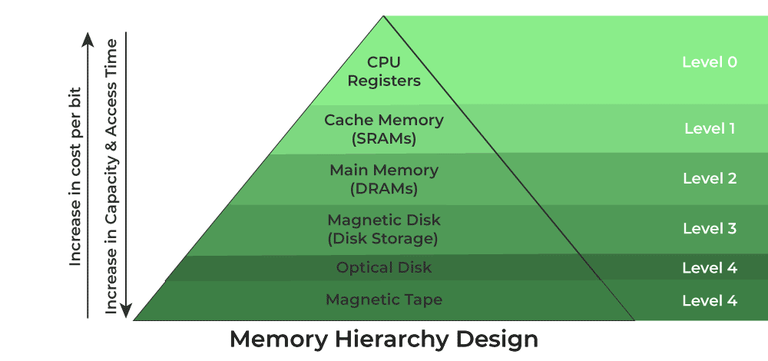
\includegraphics[width=0.7\textwidth]{memory_hierarchy.png}
    \caption{The Memory Hierarchy, illustrating the trade-off between speed, cost, and capacity. Data is moved up the pyramid to be closer to the CPU for faster access. These steps will be explained more at \ref{subsec:memory_hierarchy}}
    \label{fig:memory_hierarchy}
\end{figure}

The two primary categories of memory are:
\begin{description}
    \item[Non-Volatile Memory] This type of memory retains its information even when not powered. It is used for long-term, permanent storage. Examples include hard disk drives (HDDs), solid-state drives (SSDs), and flash drives.
    \item[Volatile Memory] This memory loses all its data when power is removed. It is used for active, in-progress tasks due to its high speed. Examples include the CPU's registers and the main system Random Access Memory (RAM).
\end{description}
For instance, an operating system and its applications are stored permanently on a large, economical hard drive (non-volatile), but when a program is run, it is loaded into the much faster, smaller, and more expensive RAM (volatile). A smaller, even faster cache built into the CPU holds the most frequently used data for immediate access.

\subsubsection{Data Transfer Mechanisms}
For a computer to function, its components must be able to communicate. The ALU must connect to the registers, and both must connect to memory. This is accomplished using a special pathway called a \textbf{bus}. A bus is a set of parallel electrical conductors that transfers data between components. The data transfer process involves three key steps:
\begin{enumerate}
    \item \textbf{Device Selection:} Identifying the source and destination devices for the transfer.
    \item \textbf{Address Selection:} Specifying the exact memory location to read from or write to.
    \item \textbf{Data Transfer:} Moving the actual data across the data bus.
\end{enumerate}

\begin{figure}[h]
    \centering
    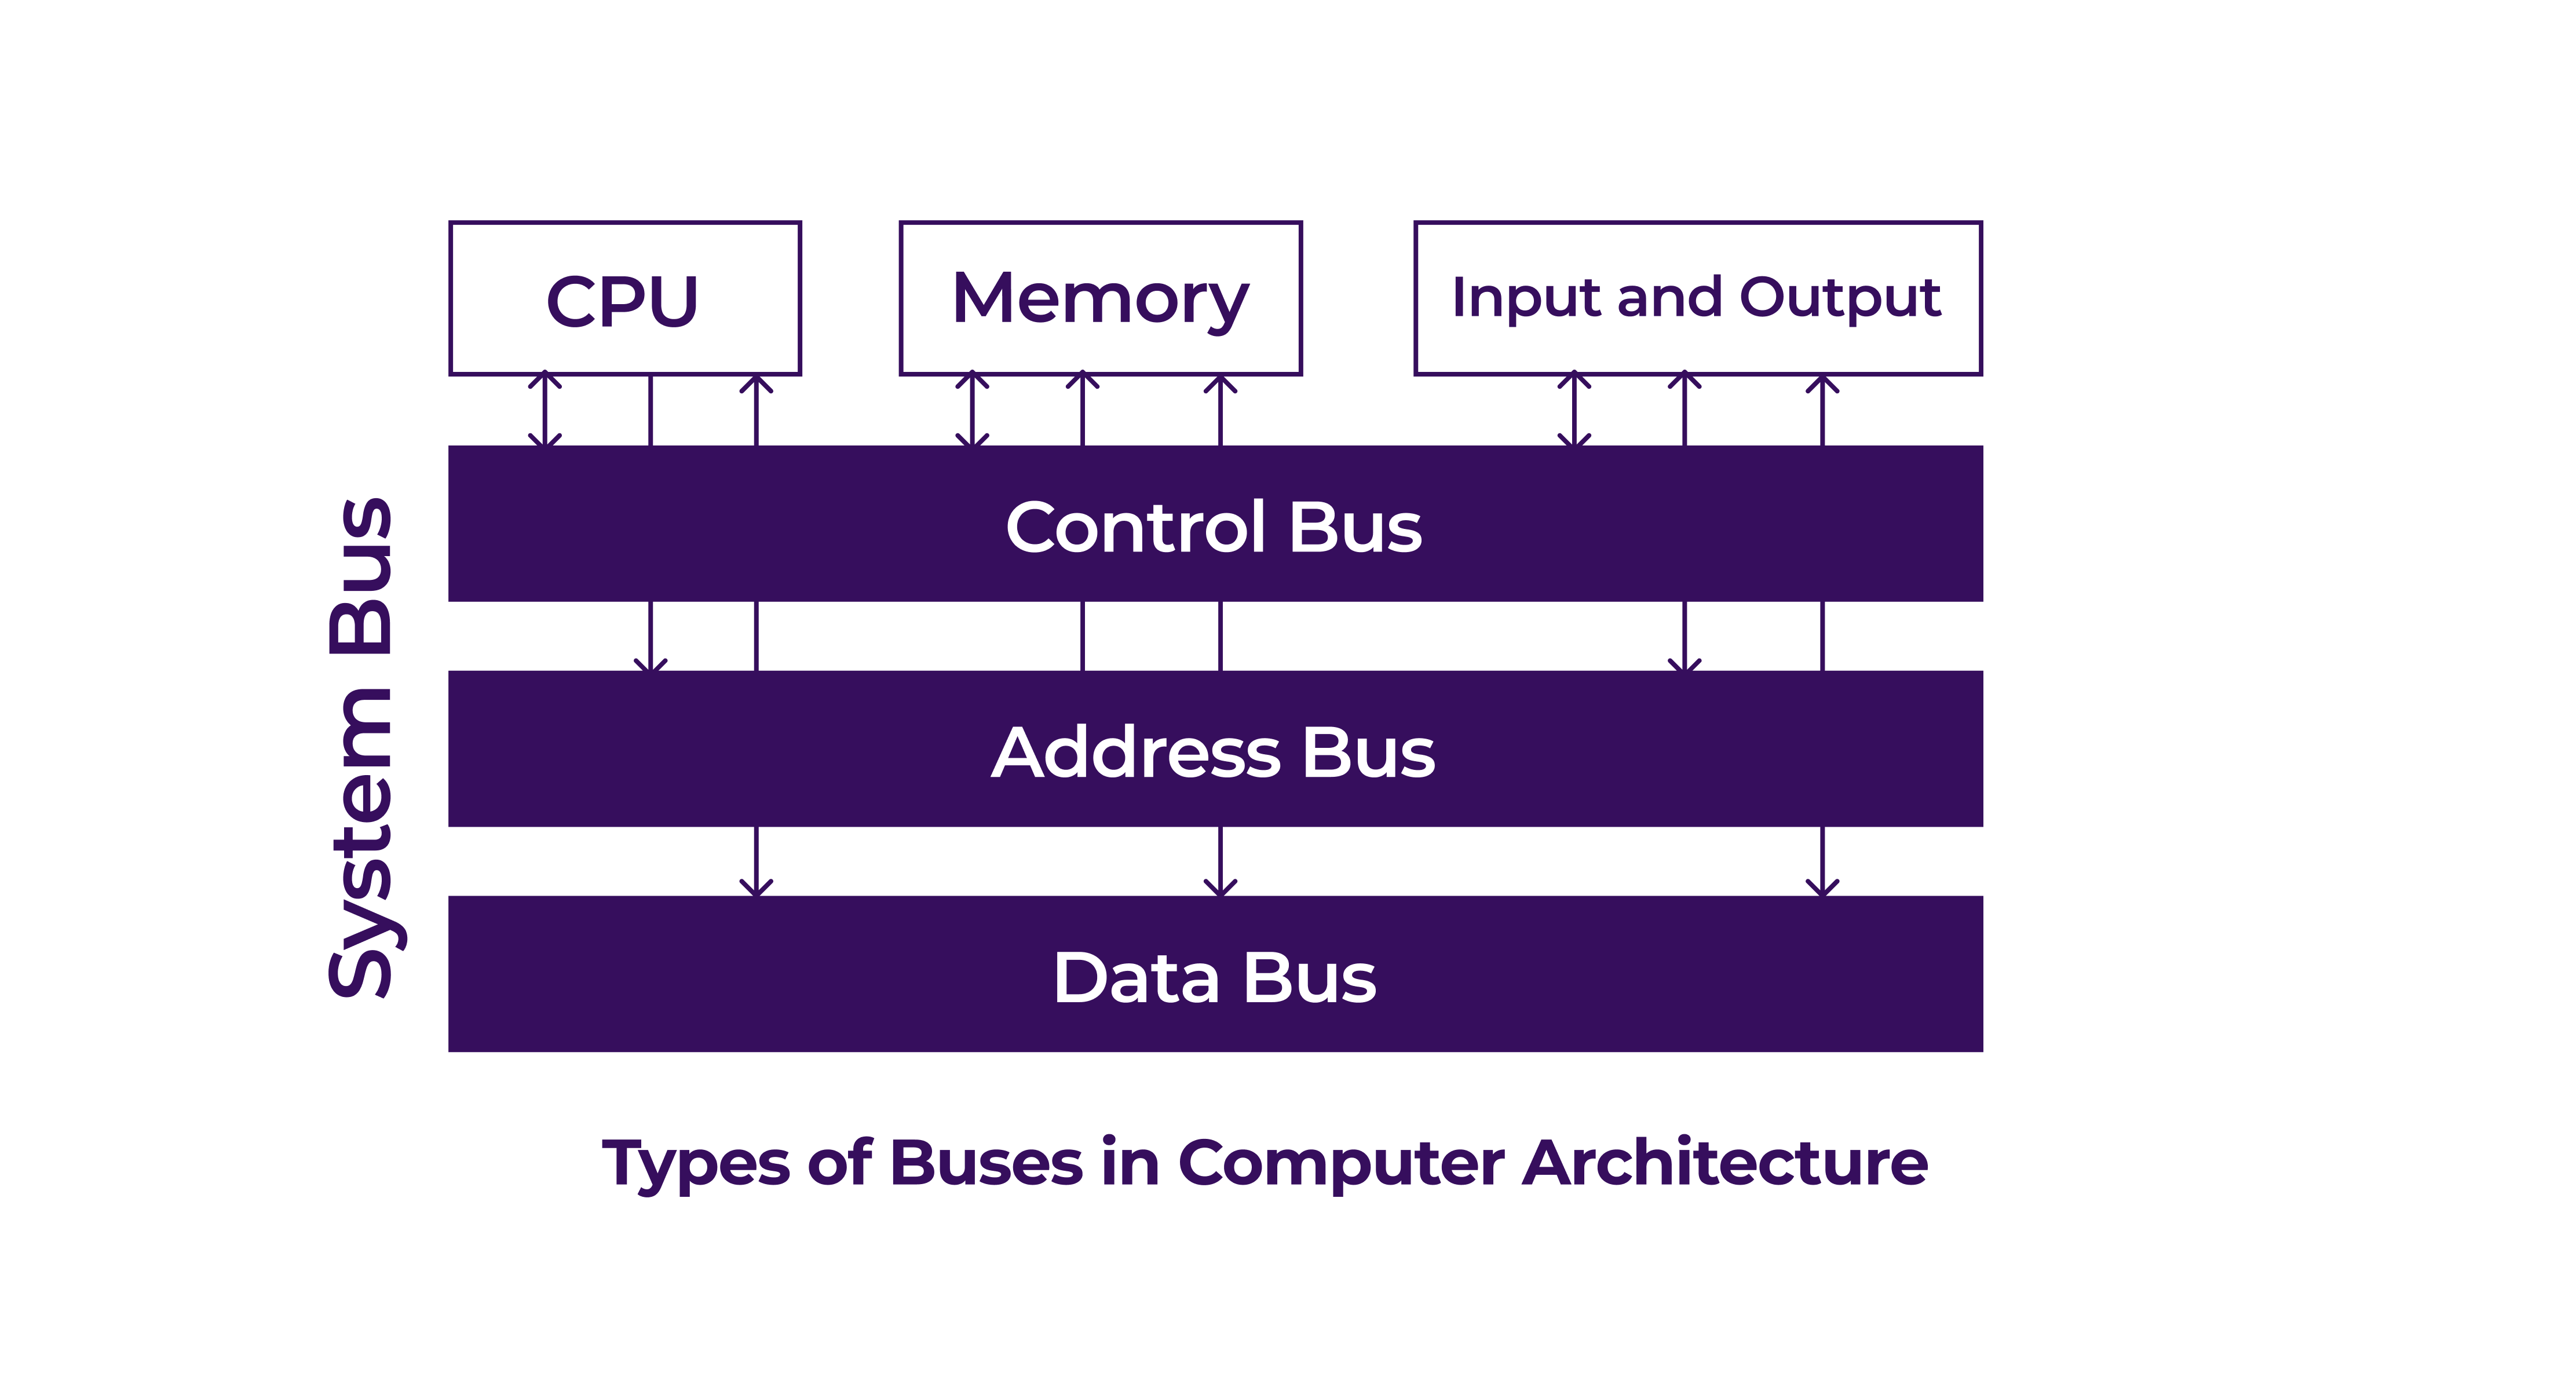
\includegraphics[width=0.75\linewidth]{buses.png}
    \label{fig:placeholder}
\end{figure}

\subsubsection{The Complete System: Hardware and Software}
While the term "computer" often refers only to the hardware, a complete \textbf{computer system} is the combination of hardware and software. The most important software is the \textbf{system software}, which includes the \textbf{operating system (OS)}. The OS acts as the crucial interface between the user and the computer's hardware. Other software categories include:
\begin{description}
    \item[Application Software] Programs used for specific end-user tasks, such as email clients or word processors.
    \item[Utility Software] Programs that help manage and maintain the computer, such as antivirus software or disk cleanup tools.
\end{description}
Peripherals like keyboards, mice, monitors, and printers are also considered part of the overall computer system. In contemporary computing, smartphones, tablets, and smartwatches can also become part of the system when they are linked to a computer.

\subsubsection{Classification of Computing Devices}
Computer systems come in a vast range of sizes and power levels. They can be broadly classified into the following categories:

    \textbf{Supercomputers or Server Clusters:} These are large-scale computing systems composed of many individual servers (nodes) connected by a high-speed network, designed to achieve massive performance and reliability for scientific and engineering problems.
    \begin{itemize}
        \item \textbf{Example: El Capitan Supercomputer}
        \item \textbf{Speed:} Approximately 2.7 exaFLOPS ($2.7 \times 10^{18}$ 64-bit floating-point operations per second). For perspective, the human brain is estimated to perform at a comparable scale of around 1 exaFLOP.
        \item \textbf{Hardware:} Comprises 11,039,168 cores, combining AMD EPYC CPUs and AMD Instinct MI300A APUs (which merge CPU and GPU cores).
        \item \textbf{Memory:} Approximately 11.4 PB of total RAM.
        \item \textbf{Network:} Slingshot-11 interconnect, with speeds of 200 Gbps.
        \item \textbf{Power:} Consumes nearly 30 Megawatts.
        \item \textbf{Operating System:} TOSS (Tri-Lab Operating System Stack), based on Red Hat Enterprise Linux.
    \end{itemize}

    \begin{figure}[h]
        \centering
        \includegraphics[width=0.75\linewidth]{The Supercomputer DeepSouth: the World's First Neuromorphic Supercomputer.png}
        \caption{The Supercomputer DeepSouth: the World's First Neuromorphic Supercomputer}
        \label{fig:placeholder}
    \end{figure}
    
    \textbf{Mainframes:} 
    \begin{wrapfigure}{r}{0.45\textwidth} % r=right, 0.45\textwidth=width
        \vspace{-20pt} % Optional: Adjust vertical spacing to pull the image up
        \centering
        \includegraphics[width=\linewidth]{IBM Mainframe.png}
        \caption{An IBM z-series Mainframe.}
        \label{fig:mainframe}
        \vspace{-10pt} % Optional: Adjust spacing below the image
    \end{wrapfigure}
    These are large, powerful, single-computer systems used by large organizations for critical applications requiring high-volume transaction processing. Unlike a server cluster, which is a collection of many machines, a mainframe is a monolithic, highly reliable unit. They are commonly used for airline ticket reservations, banking transactions, and other mission-critical tasks.

    \textbf{Personal Computers (PCs):} This category includes desktops and laptops. Although portable devices have become immensely popular, desktops often provide better performance-per-dollar and can be more ergonomic for workers.\\

    \textbf{Mobile Devices:} This includes any handheld portable computing device, such as a smartphone or tablet. They are typically used for communication, photography, and accessing web content.\\

    \textbf{Embedded Systems:} These are specialized computer systems designed for a specific function within a larger mechanical or electrical system. They are ubiquitous, found in everything from greeting cards and automotive engine control units to industrial machinery. They are often mass-produced and cost-optimized.

\subsection{Measurement Terminology in Computer Science}
\label{subsec:measurement_terminology}

A significant point of confusion in computer science arises from the dual use of prefixes such as "kilo," "mega," and "giga." Depending on the context, these terms can refer to powers of 10 (the decimal system) or powers of 2 (the binary system), leading to ambiguity in representing data storage and transmission rates.

To resolve this, the \textbf{International Electrotechnical Commission (IEC)}, with support from organizations like the National Institute of Standards and Technology (NIST), established a standard set of names and symbols for binary prefixes. This standard provides a clear and unambiguous way to differentiate between the two systems.

The distinction is summarized in the table below. The decimal (SI) prefixes are commonly used in networking and are often used by storage manufacturers for marketing purposes, while the binary (IEC) prefixes accurately represent data capacity in powers of 2, which is how computer memory is addressed.

\begin{table}[h!]
    \centering
    \caption{Comparison of Decimal (SI) and Binary (IEC) Prefixes.}
    \label{tab:si_vs_iec_prefixes}
    \begin{tabular}{|l|c|l||l|c|l|}
        \hline
        \multicolumn{3}{|c||}{\textbf{Decimal System (SI)}} & \multicolumn{3}{c|}{\textbf{Binary System (IEC)}} \\
        \hline
        \textbf{Name} & \textbf{Symbol} & \textbf{Value} & \textbf{Name} & \textbf{Symbol} & \textbf{Value} \\
        \hline
        Kilobyte & kB & $10^3$ & Kibibyte & KiB & $2^{10}$ \\
        Megabyte & MB & $10^6$ & Mebibyte & MiB & $2^{20}$ \\
        Gigabyte & GB & $10^9$ & Gibibyte & GiB & $2^{30}$ \\
        Terabyte & TB & $10^{12}$ & Tebibyte & TiB & $2^{40}$ \\
        Petabyte & PB & $10^{15}$ & Pebibyte & PiB & $2^{50}$ \\
        Exabyte & EB & $10^{18}$ & Exbibyte & EiB & $2^{60}$ \\
        Zettabyte & ZB & $10^{21}$ & Zebibyte & ZiB & $2^{70}$ \\
        Yottabyte & YB & $10^{24}$ & Yobibyte & YiB & $2^{80}$ \\
        \hline
    \end{tabular}
\end{table}

\subsubsection{Informal Conventions and Practical Application}
Prior to the widespread adoption of the IEC standard, an informal convention emerged to distinguish the bases. In this system, a lowercase prefix letter might indicate a power of 10 (e.g., 1 \textbf{kB} = 1000 bytes), while an uppercase prefix letter might indicate a power of 2 (e.g., 1 \textbf{KB} = 1024 bytes). However, this convention is not universally followed and can still lead to confusion.

A related and critical distinction is between the \textbf{bit} and the \textbf{Byte}. One Byte is composed of 8 bits. This difference is especially important in the context of data rates versus storage:
\begin{itemize}
    \item \textbf{Data Transmission Speed} is typically measured in bits per second, using decimal prefixes (e.g., kilobits per second or Kbps).
    \item \textbf{Data Storage Capacity} is typically measured in Bytes, preferably using binary prefixes for technical accuracy (e.g., KiloBytes (KB) or, more precisely, Kibibytes (KiB)).
\end{itemize}
Given the inconsistent application of these terms in commercial products, it is imperative to \textbf{consult manufacturer specifications} to determine precisely which measurement system is being used.

\subsection{Von Neumann Architecture}
Proposed by John von Neumann in 1945, this architecture is the basis for the vast majority of modern computers. Its defining feature is the concept of the \textbf{stored-program computer}.

Historically, computers were \textit{fixed-program} (like a calculator). The Von Neumann architecture introduced the revolutionary idea that both the \textbf{instructions (the program) and the data should be stored in the same main memory}.

\begin{figure}[h]
    \centering
    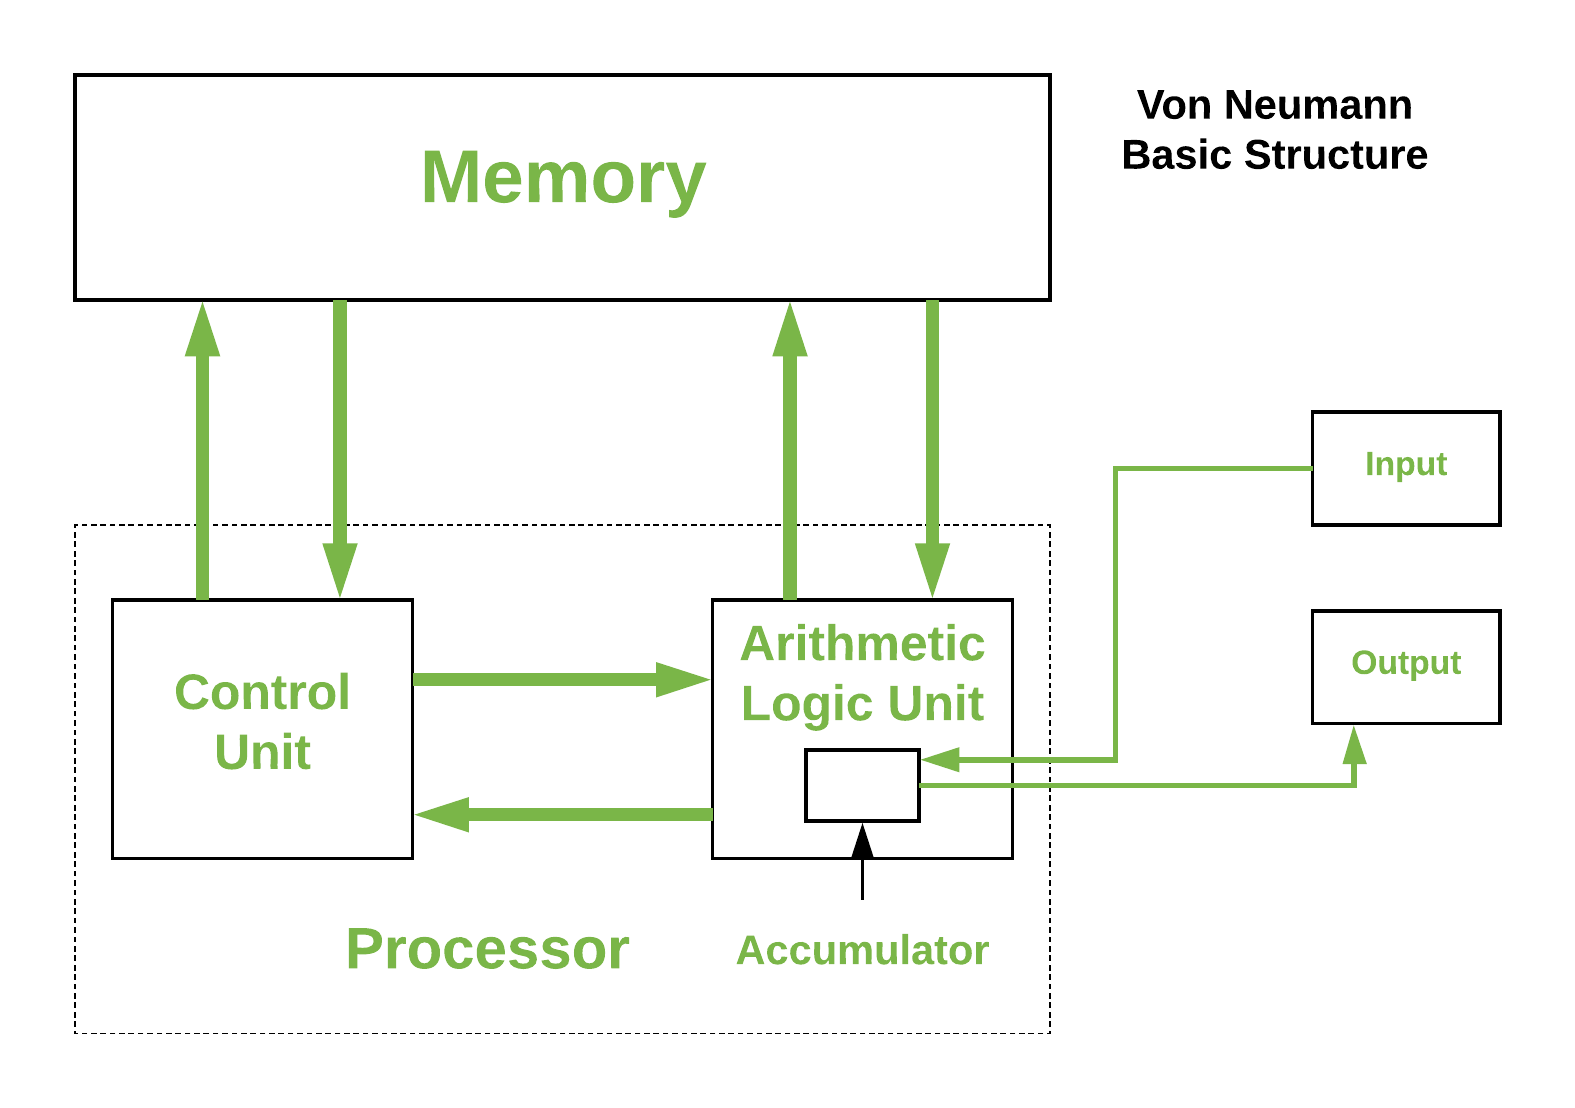
\includegraphics[width=0.75\linewidth]{Von Neumann.png}
\end{figure}

\subsection{Core Components of the Von Neumann Architecture}
\label{subsec:von_neumann_components}
The Von Neumann model organizes a computer system into a set of distinct, cooperating components. Although some of these concepts have been previously introduced, supposing this is your first approach to architectures a recapitulation is beneficial; the Central Processing Unit (CPU) and the Main Memory Unit are at the heart of this design, connected by a bus system that facilitates the transfer of both data and instructions.

\subsection*{The Central Processing Unit (CPU)}
The CPU is the active part of the computer, responsible for executing the instructions of a program. It is comprised of three principal components: the Control Unit (CU), the Arithmetic Logic Unit (ALU), and a set of registers.

\paragraph{The Control Unit (CU) and Arithmetic Logic Unit (ALU)}
The CU and ALU work in tandem to perform the computations required by a program.
\begin{description}
    \item[Control Unit (CU)] The CU acts as the orchestrator of the CPU. It does not execute instructions itself, but rather interprets them and generates control signals that direct the operations of the entire system. Its primary responsibilities include fetching instructions from memory, decoding them to determine the required action, and coordinating the flow of data between the registers, the ALU, and main memory. It manages the entire fetch-decode-execute cycle.
    
    \item[Arithmetic Logic Unit (ALU)] The ALU is the computational core of the processor. It handles all calculations the CPU may need to perform. These operations are broadly categorized into two types:
    \begin{itemize}
        \item \textbf{Arithmetic operations:} Including addition, subtraction, multiplication, and division.
        \item \textbf{Logical operations:} Including comparisons, boolean operations (AND, OR, NOT, XOR), and bit-shifting operations.
    \end{itemize}
\end{description}

\paragraph{Registers}
Registers are high-speed storage areas located directly within the CPU, sitting at the apex of the memory hierarchy. They provide the fastest way for the CPU to access data. While a processor contains many registers for various purposes, several are fundamental to the Von Neumann architecture's operation:

\textbf{Program Counter (PC):} This register holds the memory address of the next instruction to be fetched for execution. After an instruction is fetched, the PC is automatically incremented to point to the subsequent instruction, unless a jump or branch instruction explicitly modifies its value.
\par\medskip % Espacio entre párrafos

\textbf{Memory Address Register (MAR):} This register holds the memory address of the data or instruction that is to be read from or written to memory. The MAR is the sole gateway to the memory system; any location to be accessed must first have its address loaded into the MAR.

\begin{wrapfigure}{r}{0.6\linewidth}
    \vspace{-12pt} % Ajuste vertical
    \centering
    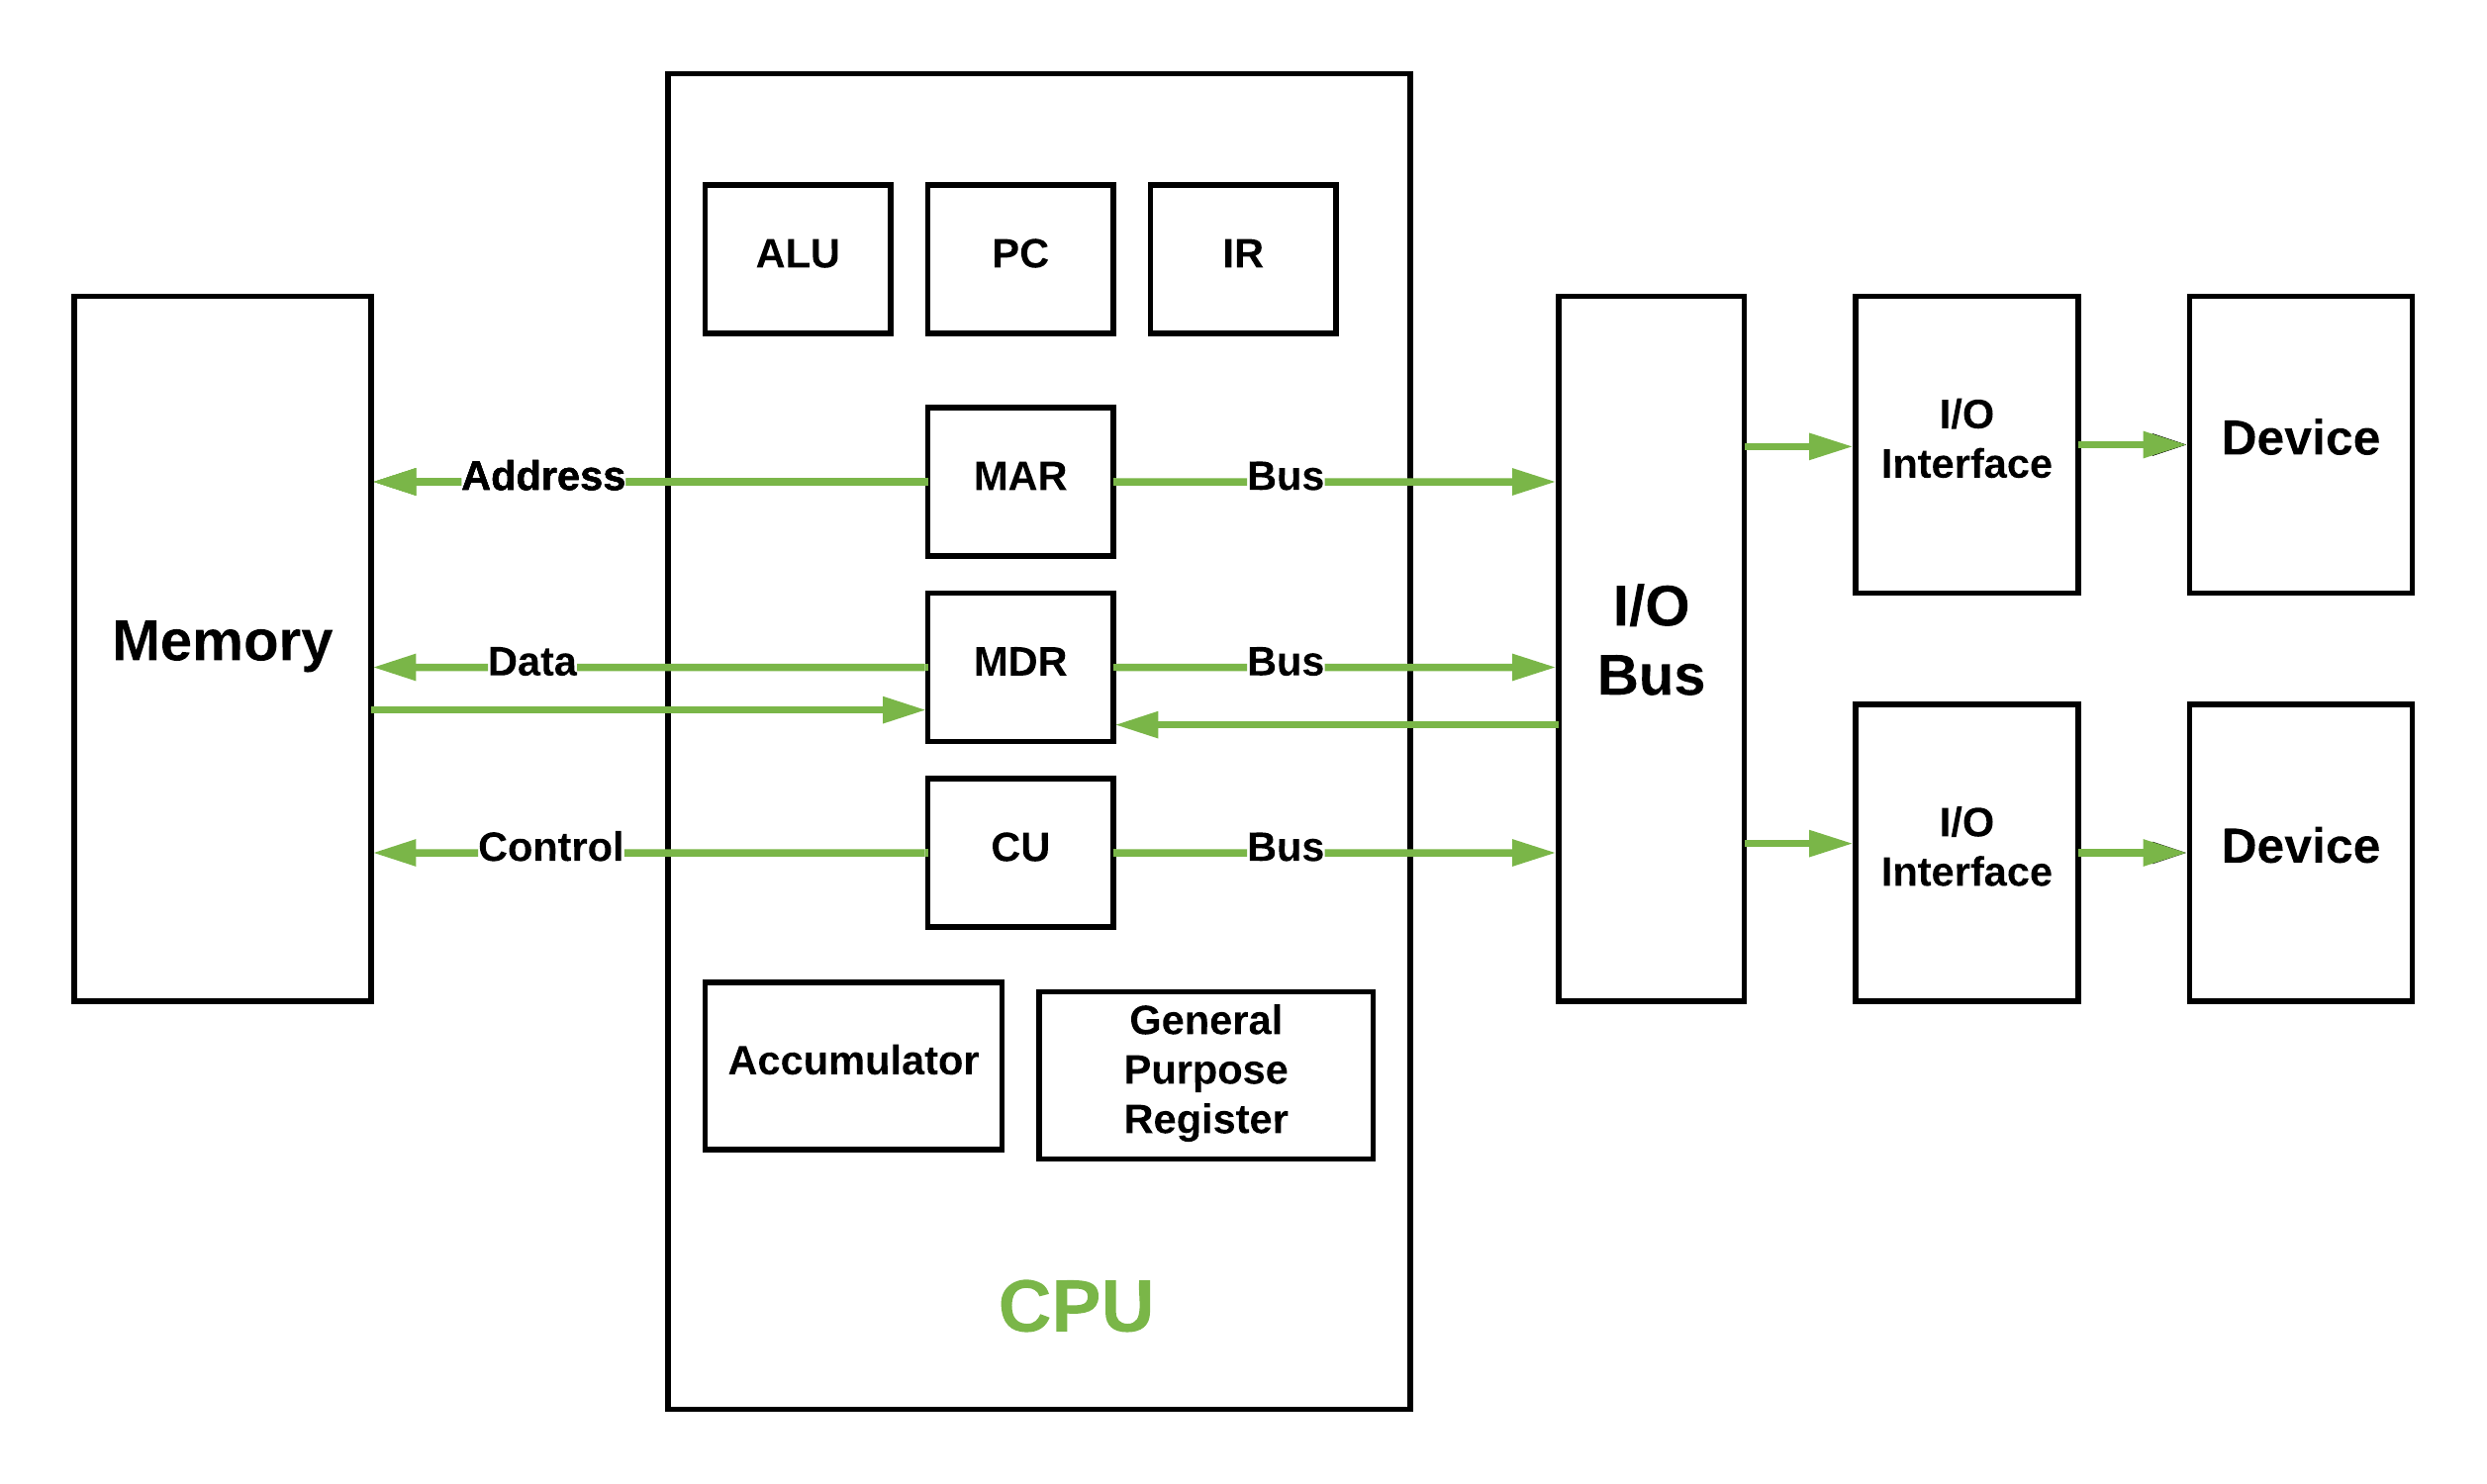
\includegraphics[width=\linewidth]{VN2.png}
    \label{fig:vn_registers_wrap}
    \vspace{-20pt} % Ajuste vertical
\end{wrapfigure}

\par\medskip
\textbf{Memory Data Register (MDR):} Also known as the Memory Buffer Register (MBR), this register acts as a two-way buffer. It holds the data that has just been read from memory or the data that is about to be written to memory. It serves as the intermediary between the CPU and the data bus.
\par\medskip

\textbf{Current Instruction Register (CIR):} After an instruction is fetched from memory, it is placed in the CIR. It holds the instruction while it is being decoded and executed by the Control Unit.
\par\medskip

\textbf{Accumulator (AC):} This is a general-purpose register that is often used to hold one of the operands for an ALU operation and to store the result of that operation. It is a temporary storage device integral to computation.

\subsection*{The Main Memory Unit}
The main memory unit is a digital system that stores both program instructions and the data upon which those instructions operate. It is conceptualized as a linear array of storage locations, each with a unique binary address.

\subsubsection*{The Memory Hierarchy}
\label{subsec:memory_hierarchy}

An ideal memory system would be infinitely large, infinitely fast, non-volatile, and available at no cost. Since such a device is not physically possible, computer architecture employs a compromise: the \textbf{memory hierarchy}. This is a structural organization of the memory system into multiple levels, designed to minimize average memory access time by creating the illusion of a large, fast memory from a combination of smaller, faster memories and larger, slower ones.

The effectiveness of this structure is predicated on the principle of \textbf{locality of reference}, a predictable tendency in program behavior. Locality manifests in two forms:
\begin{itemize}
    \item \textbf{Temporal Locality:} If a program accesses a memory location, it is highly probable that it will access the same location again in the near future.
    \item \textbf{Spatial Locality:} If a program accesses a memory location, it is highly probable that it will also access nearby memory locations soon.
\end{itemize}

\paragraph{Cache Operation and Challenges}
The effectiveness of the hierarchy is based on the operation of the cache memory. When the CPU needs a piece of data, it first looks in the cache. If the data is found there, a \textbf{cache hit} occurs, which is an extremely fast operation. If it is not found, a \textbf{cache miss} occurs, and the system must fetch the data from the main memory (RAM), which is much slower. A block of memory containing the requested data (and adjacent data, leveraging spatial locality) is then copied into the cache. Thanks to the principle of locality, the probability of future hits is very high, making the \textit{average} memory access time much closer to that of the cache than that of RAM.

In multi-core systems, this hierarchy introduces a fundamental challenge: \textbf{cache coherence}. If each core has its own private cache, it is possible for multiple copies of the same data to exist. If one core modifies its copy, the others become stale, which can lead to incorrect results. To prevent this, processors implement complex cache coherence protocols (such as MESI) to ensure that all cores have a consistent view of memory.

By placing recently or frequently used data in the faster, higher levels of the hierarchy, the system can satisfy the majority of memory requests without accessing the slower, lower levels, thus reducing the effective access time at a reasonable cost.

The primary levels of the memory hierarchy, from fastest to slowest, are as follows (remember \ref{fig:memory_hierarchy}):

\subsubsection{Level 0: CPU Registers}
Registers are the highest level of the hierarchy, located directly on the processor die. They are the fastest and most expensive memory available, providing the CPU with immediate access to operands and results. Their capacity is extremely limited.

\subsubsection{Level 1: Cache Memory}
Cache is a small, fast memory buffer situated between the CPU and the main memory. Its purpose is to hold copies of the most frequently used data and instructions from the main memory. Cache is almost always implemented using \textbf{Static RAM (SRAM)}.
\begin{description}
    \item[SRAM (Static RAM)] This type of memory stores each bit using a bistable latching circuit, typically composed of six transistors. The term "static" refers to the fact that it retains its state as long as power is supplied and does not need to be periodically refreshed. This design makes it significantly faster than DRAM but also less dense and more expensive per bit. Modern CPUs contain multiple levels of cache (L1, L2, and L3), each with a different size and speed trade-off. Cache is not typically user-replaceable.
\end{description}

\subsubsection{Level 2: Main Memory}
The main memory, or primary storage, is the principal workspace for a program. It is significantly larger than cache but also slower. This level is implemented using \textbf{Dynamic RAM (DRAM)}.
\begin{description}
    \item[DRAM (Dynamic RAM)] This memory stores each bit as a charge within a tiny capacitor, paired with a single transistor. The term "dynamic" arises because the capacitor leaks charge over time and must be constantly refreshed hundreds of times per second to retain its data. This refresh cycle adds overhead, making DRAM slower than SRAM. However, its simple cell structure allows for much higher storage densities and a lower cost per bit, making it suitable for large-capacity main memory modules.
\end{description}

\subsubsection{Level 3: Secondary Storage}
This level consists of non-volatile storage that retains data after power is removed. It is where the operating system, applications, and user files are stored permanently. It is much larger and slower than main memory. Examples include Hard Disk Drives (HDDs) and Solid-State Drives (SSDs). Intuitively, magnetic tapes as shown in the figure are part of.

\subsubsection{Level 4: Tertiary Storage}
Also known as offline or archival storage, this is the slowest and least expensive level, used for long-term data backup. Examples include magnetic tape libraries and cloud storage services.

\subsubsection*{Aditional data}
\begin{definition}
    \item[Word] A \textbf{word} is the natural unit of data for a particular processor architecture. It is a fixed-size group of bits (e.g., 32 or 64) that are handled as a single unit by the instruction set and/or hardware of the processor.
    
    \item[Byte] A group of 8 bits is called a \textbf{byte}. In most modern architectures, the byte is the smallest addressable unit of memory.
    
    \item[Addressability] The capacity of the memory system is determined by the width of the address bus. For a system with $k$ address lines, it is possible to uniquely address $2^k$ memory words.
\end{definition}

A consequence of this architecture is the so-called \textbf{Von Neumann bottleneck} (more details on \ref{Neumann_Bottleneck}): the bus connecting the CPU to memory is a shared resource that can become saturated, as both instructions and data must travel through it, limiting the system's performance.

\subsection{Flynn's Taxonomy}
In 1966, Michael J. Flynn proposed a taxonomy to classify computer architectures based on the number of instruction streams and data streams they can process simultaneously.

\begin{description}
    \item[SISD (Single Instruction, Single Data):] A single instruction stream operates on a single data stream. These are traditional sequential computers.
    \item[SIMD (Single Instruction, Multiple Data):] A single instruction is applied simultaneously to multiple data streams. The quintessential example is \textbf{GPUs}.
    \item[MISD (Multiple Instruction, Single Data):] Multiple instructions operate on a single data stream. It is an uncommon architecture in practice.
    \item[MIMD (Multiple Instruction, Multiple Data):] Multiple instruction streams operate on multiple data streams. This is the architecture of \textbf{multicore} processors and clusters.
\end{description}

\paragraph{The Hybrid Reality of Modern Processors}
It is important to note that the pure architectures described by Flynn are rare in contemporary hardware. A modern processor, such as an Intel Core i9 or an AMD Ryzen, is actually a complex \textbf{hybrid} system. At the level of its multiple cores, it operates as a \textbf{MIMD} machine, as each core can execute a different stream of instructions on different data independently. However, within each core are highly potent \textbf{SIMD} processing units (implemented through instruction sets like AVX or SSE), which apply a single instruction to multiple data to accelerate vector-based computational tasks. This combination shows how Flynn's theoretical concepts are integrated to maximize performance in the real world.

\begin{figure}[h]
    \centering
    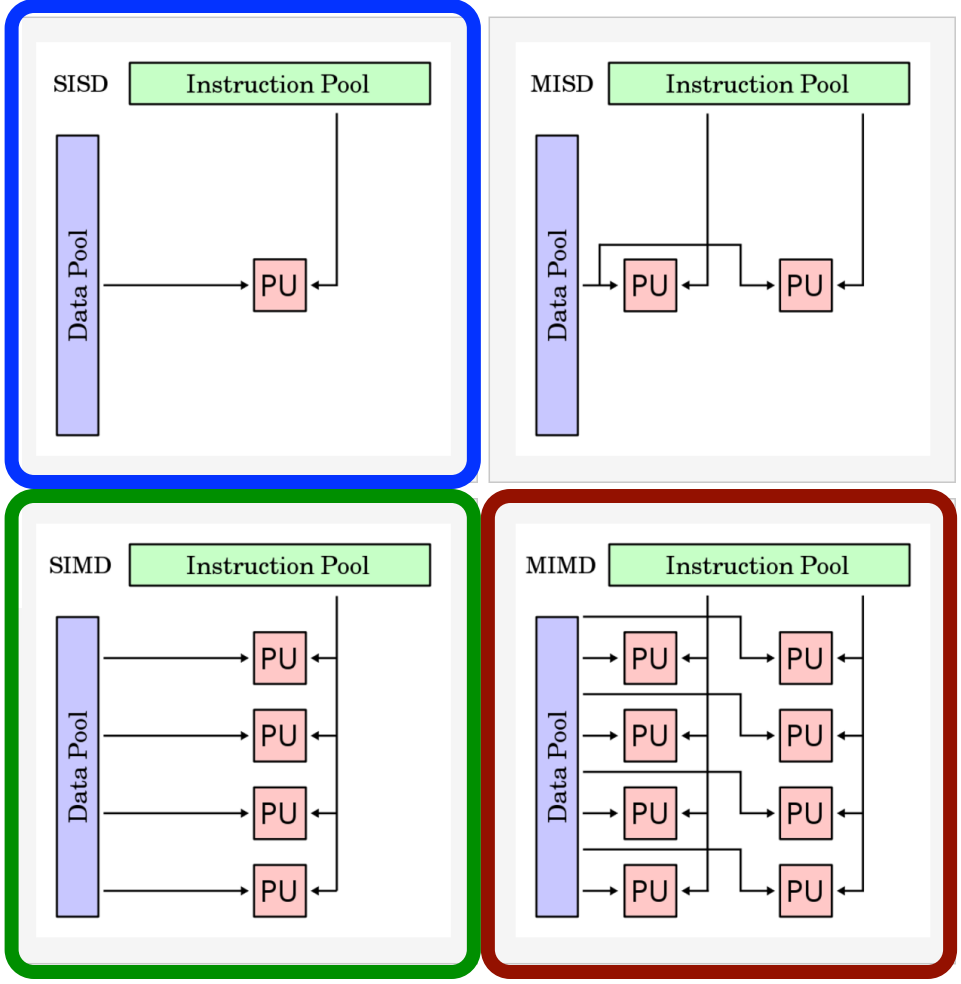
\includegraphics[width=0.75\linewidth]{XIXM.png}
    \label{fig:placeholder}
\end{figure}

\paragraph{Example: Sequential Summation}
Consider a simple loop designed to sum all elements of a list. The program iterates through each element, adding it to a running total one at a time.

\begin{lstlisting}[language=C, label={lst:seq_sum}]
list = [2, 4, 6, 8];
n = 4;
int sum = 0;
for (int i = 0; i < n; i++) {
    sum += list[i];
}
print(sum);
\end{lstlisting}

The execution trace for this algorithm is strictly sequential:
\begin{lstlisting}[language=C, label={lst:seq_sum2}]
sum = 0
sum = sum + list[0]  // sum becomes 2
sum = sum + list[1]  // sum becomes 6
sum = sum + list[2]  // sum becomes 12
sum = sum + list[3]  // sum becomes 20
...
\end{lstlisting}
This operation requires $n$ additions and its execution time, $T(n)$, is directly proportional to $n$. We can recognize that the summation can be decomposed; for instance, by adding pairs of numbers independently and then summing the partial results. However, with a single processor, this architectural change offers no performance gain. The same number of additions must be performed in the same total amount of time.

The true performance benefit is unlocked only when multiple processing units are available. If we had $n/2$ processors, we could perform many of the calculations simultaneously, drastically reducing the execution time while performing the same number of total operations. This fundamental insight is the motivation for concurrent, parallel, and distributed computing.

\subsection{Fundamental Terminology}
To properly discuss these \textit{paradigms}, we must first define the core concepts.\\

\hline
\textbf{The Concept of a Paradigm}. Due to Programming and paradigms for DS I would like to introduce formally the term \textbf{paradigm}, derived from the Greek \textit{paradeigma} (\foreignlanguage{greek}{παράδειγμα}), meaning "pattern" or "model," refers to a fundamental framework of concepts, theories, and practices that constitutes a way of viewing reality. In a broader scientific context, as defined by the philosopher Thomas Kuhn, a paradigm represents a set of universally recognized scientific achievements that, for a time, provide model problems and solutions to a community of practitioners. A \textbf{paradigm shift} occurs when the existing framework is no longer adequate to explain new phenomena, leading to a scientific revolution and the adoption of a new model.

In computer science, this concept is applied to define a \textbf{programming paradigm}: a fundamental style or approach to building computer programs. It is not a specific language but rather a way of thinking about and structuring computation itself.

The models of computation discussed herein represent such a paradigm shift.
\begin{itemize}
    \item The \textbf{Sequential Paradigm} was the dominant model for decades. It frames computation as a single, linear sequence of instructions executed one after another. Algorithmic design within this paradigm is focused on optimizing this single timeline.
    
    \item The move toward \textbf{Concurrent, Parallel, and Distributed Processing} represents a fundamental paradigm shift. It reframes computation not as a single timeline, but as a collection of multiple, interacting processes or threads. This shift was necessitated by physical limitations in processor speed and the increasing complexity of problems to be solved. Adopting this new paradigm requires a different way of thinking, introducing new fundamental challenges such as synchronization, communication, and consistency, which are non-existent in the sequential model.
\end{itemize}
\hline

\subsection{Fundamental Concurrency Primitives}
Beyond the general concepts of processes and threads, the practical implementation of concurrent systems relies on a set of fundamental primitives provided by the operating system and programming language runtimes. Two of the most foundational are the \texttt{fork()} system call for process creation and the mechanism of \textbf{condition variables} for advanced thread synchronization.

\paragraph{The \texttt{fork()} System Call}
The \texttt{fork()} system call is the primary method for creating new processes in UNIX-like operating systems. It creates a new process, termed the \textit{child process}, by duplicating the calling process, termed the \textit{parent process}. The child process is an almost exact copy of the parent; it inherits copies of the parent's address space, file descriptors, and other context information.

The defining characteristic of \texttt{fork()} is its return value. Upon successful completion, \texttt{fork()} returns:
\begin{itemize}
    \item A value of \textbf{0} to the child process.
    \item The \textbf{Process ID (PID)} of the newly created child process to the parent process.
\end{itemize}
This differentiation in return values is the fundamental mechanism that allows the two processes to follow distinct execution paths after the call. A canonical usage pattern is as follows:

\begin{lstlisting}[language=C, caption={Canonical usage of the fork() system call}]
pid_t pid = fork();

if (pid < 0) {
    // Fork failed; an error occurred.
    fprintf(stderr, "Fork Failed");
    return 1;
} else if (pid == 0) {
    // This block is executed by the child process.
    printf("Executing child process code\n");
    execlp("/bin/ls", "ls", NULL); // Example: child replaces its image
} else {
    // This block is executed by the parent process.
    printf("Parent process, child PID is %d\n", pid);
    wait(NULL); // Parent waits for the child to complete.
    printf("Child Complete");
}
\end{lstlisting}

This primitive is the low-level foundation for the behavior of Python's \texttt{multiprocessing} module on POSIX-compliant systems, where a new interpreter process is forked to achieve true parallelism.

\paragraph{Condition Variables and the Notify Mechanism}
While a lock (mutex) provides mutual exclusion, it does not offer a mechanism for threads to wait for a specific \textit{condition} to become true without resorting to inefficient busy-waiting. This capability is provided by \textbf{condition variables}.

A condition variable is a synchronization object that is always associated with a mutex. It allows threads to suspend their execution atomically until some condition, predicate $P$, on the shared data is satisfied. It supports three primary operations:
\begin{itemize}
    \item \texttt{wait()}: This operation must be called while holding the associated mutex. It atomically releases the mutex and suspends the execution of the calling thread. When the thread is later awakened, it re-acquires the mutex before \texttt{wait()} returns. The atomicity is crucial to prevent lost wake-ups. Because a thread might be awakened spuriously, the condition $P$ must be re-checked in a loop.
    \item \texttt{notify()} (or \texttt{signal()}): This operation, called by a thread that holds the mutex and has just changed the state such that $P$ may now be true, awakens \textit{at least one} of the threads currently waiting on the condition variable.
    \item \texttt{notifyAll()} (or \texttt{broadcast()}): This is similar to \texttt{notify()}, but it awakens \textit{all} threads currently waiting on the condition variable. The awakened threads will then contend for the mutex to re-check the condition $P$. This is used when multiple waiting threads might be able to proceed or to simplify logic, though it can introduce a "thundering herd" problem where many threads wake only to find they cannot proceed.
\end{itemize}
Condition variables are the essential building block for solving canonical concurrency problems, such as the Producer-Consumer problem, in an efficient, non-blocking manner.

A \textbf{program} is a static set of instructions, typically stored in a file on a long-term storage system. It represents a passive entity, containing the code to perform one or more \textit{tasks}. Examples include web browsers, text editors, and database management systems.\\
    
A \textbf{process} is a program in execution. It is an active entity to which the operating system allocates resources, such as a private memory address space, file handles, and environment variables. Each process has its own independent state and is isolated from other processes on the system.\\
    
A \textbf{task} is a set of program instructions loaded into memory for execution. It represents a unit of work that the operating system's \textbf{scheduler} assigns to a programmable entity, known as a thread.\\

\vspace{3cm}

\begin{wrapfigure}{l}{0.5\linewidth} % l=left, 0.5\linewidth=width
    \vspace{-15pt} % Optional: Adjusts vertical spacing
    \centering
    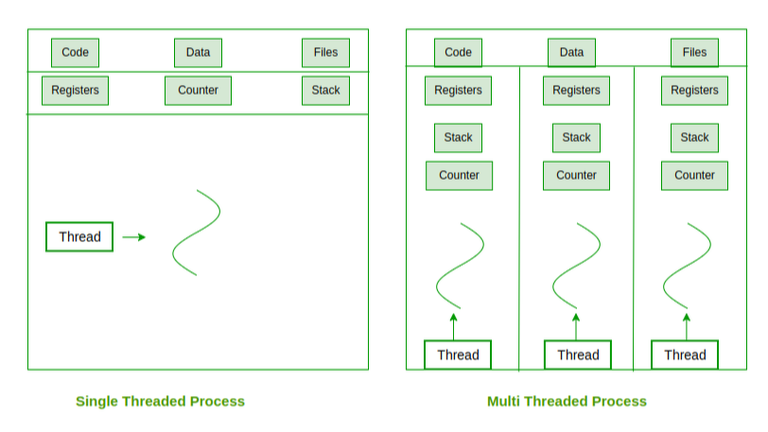
\includegraphics[width=\linewidth]{thread.png}
    \caption{A process with multiple threads sharing memory.}
    \label{fig:multithreaded_process}
    \vspace{-10pt} % Optional: Adjusts vertical spacing
\end{wrapfigure}

A \textbf{thread} (also known as a lightweight process) is the smallest unit of execution that an operating system can schedule. It represents a single, concurrent path of execution that results from a program forking or bifurcating into two or more tasks. 

A single process can contain multiple threads, all of which operate within the same memory context. These threads share the process's resources, including its memory address space, code segment, open files, timers, and \textbf{counters} (generally, a \underline{device} or variable used to store and track the number of times an event has occurred). This resource sharing is a key distinction from processes, which are typically isolated from one another and do not share memory by default.

However, to allow for independent execution, each thread maintains its own private context. This private context includes a program counter, a set of registers, and a \textbf{stack}, which is a dedicated memory area used to manage its active function calls and store local variables. This hybrid model allows for efficient communication between threads (via shared memory) while enabling them to execute different instruction sequences concurrently.

Practical examples of multithreading are ubiquitous. For instance, a word processor might use one thread to respond to user input, while separate background threads perform tasks like automatic spell-checking and auto-saving simultaneously.

\subsubsection{Task States}

\begin{wrapfigure}{r}{0.5\linewidth}
    \vspace{-15pt} % Adjust vertical spacing
    \centering
    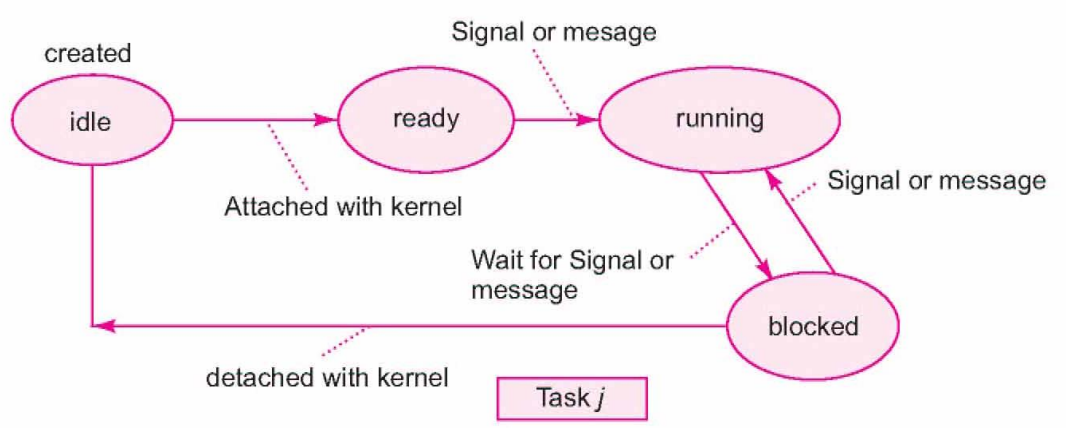
\includegraphics[width=\linewidth]{thread states.png}
    \caption{A diagram illustrating the primary states of a task or thread.}
    \label{fig:task_states}
    \vspace{-10pt}
\end{wrapfigure}

As a task is managed by the operating system, it transitions between several states:

\par\medskip\noindent
\textbf{Idle (or New):} The task has just been created or has been blocked for an extended period and moved out of the active queue.

\par\medskip\noindent
\textbf{Ready:} The task has all the resources it needs to run and is waiting to be assigned to a processor core by the scheduler.

\par\medskip\noindent
\textbf{Running:} The task is currently being executed by a processor core.

\par\medskip\noindent
\textbf{Blocked:} The task cannot proceed because it is waiting for a resource to become available or for an event to occur (e.g., an I/O operation to complete). Once the event occurs, it transitions back to the Ready state.

\subsubsection{Computability versus Computational Complexity}
It is important to distinguish between two related fields of study:
\begin{description}
    \item[Computability Theory] This field focuses on whether a problem can be solved by an algorithm at all, without regard for the resources required to do so. It is concerned with the fundamental limits of what can be computed.
    \item[Computational Complexity Theory] This field is concerned with the quantity of resources required to solve a problem. Commonly studied resources include execution time, number of operations, number of processor cores, memory usage, storage space, and network bandwidth.
\end{description}

\subsection{Processing Paradigms}
With this terminology established, we can now formally define the different processing paradigms.

\begin{wrapfigure}{r}{0.5\linewidth}
    \centering
    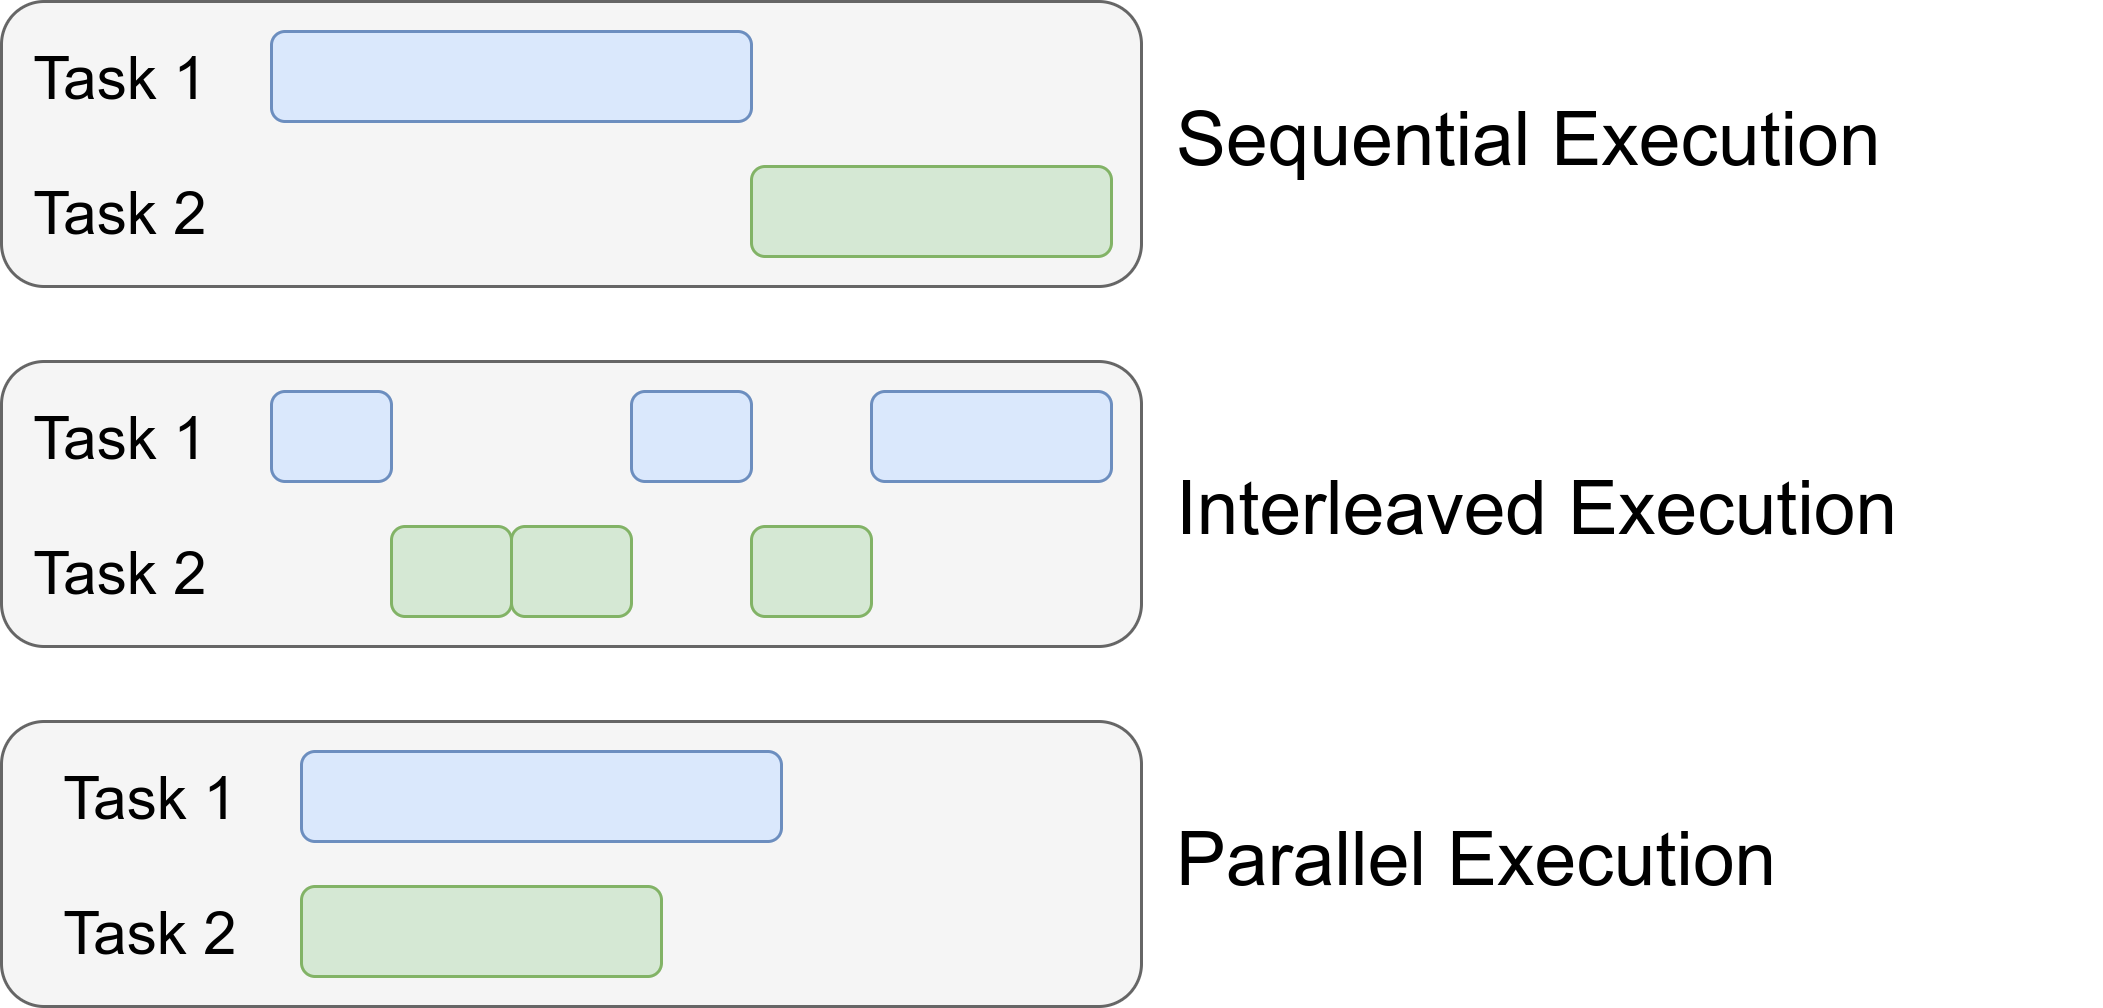
\includegraphics[width=\linewidth]{Seq, conc & parall.png}
    \caption{Processing Paradigms.}
    \label{fig:computation_models}
\end{wrapfigure}

\noindent
\textbf{Sequential Processing:} The traditional model of computation where instructions are executed one after another, in a single stream, on a single processor. Only one instruction is executed at any given moment.

\par\medskip\noindent
\textbf{Concurrent Processing:} Concurrency is the property of an algorithm or system that allows it to be decomposed into separate pieces that can be managed out of order or in partial order without affecting the final outcome. It is a \textbf{design concept}. A concurrent program can be executed on a single processor through time-slicing (creating the illusion of simultaneity), or on multiple processors.

\begin{wrapfigure}{l}{0.5\linewidth}
    \centering
    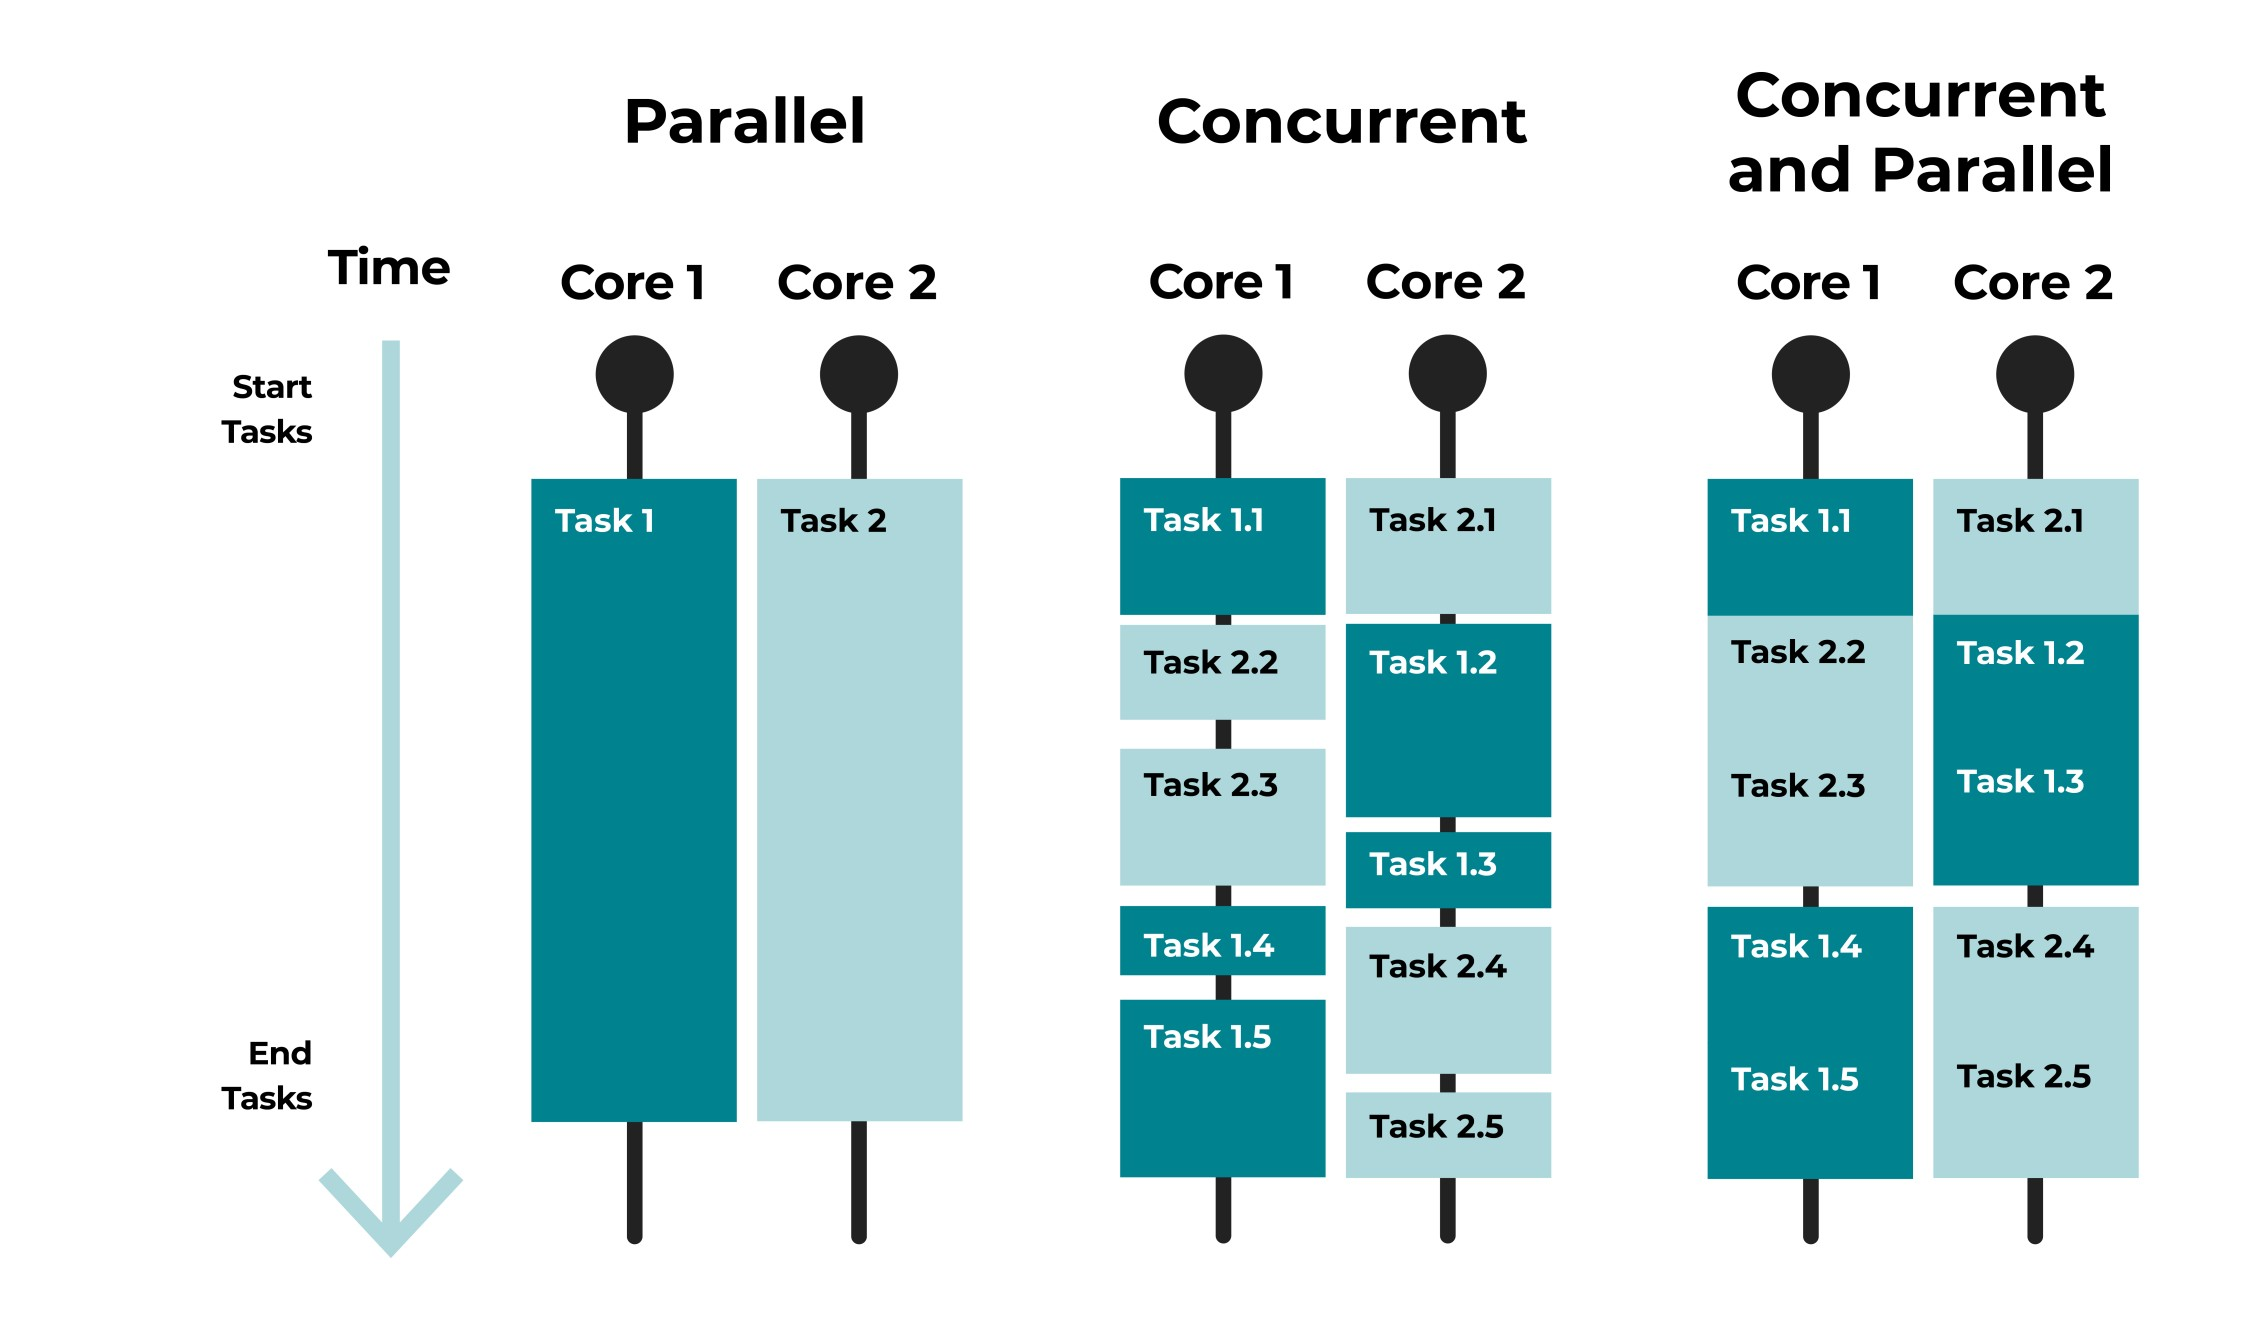
\includegraphics[width=\linewidth]{cvsp.png}
    \caption{Concurrency vs Parallelism.}
    \label{fig:computation_models}
\end{wrapfigure}

\par\medskip\noindent
\textbf{Parallel Processing:} Parallelism is the mechanism used to execute a concurrent program on a multi-processor architecture to improve performance. It is the \textbf{simultaneous execution} of two or more threads or processes. The performance gain is often measured by \textbf{speedup}, calculated as the ratio of sequential execution time to parallel execution time. For example, if a sequential solution takes 60 minutes and a parallel solution takes 6 minutes, the speedup is 10.

\par\medskip\noindent
\textbf{Distributed Processing:} This refers to parallel processing that is distributed across multiple, independent computing devices that communicate over a network to solve a single problem. While this can greatly improve performance, it introduces significant \textbf{communication overhead}. For a distributed solution to be worthwhile, the time saved by distributing the operations must be greater than the time added by network communication latency. This is a critical consideration in designing distributed systems, such as those used for training large deep learning models.

\section{A little deeper Concepts in Parallel and Distributed Computing}
\label{sec:advanced_parallel_concepts}

Designing efficient parallel programs requires more than just understanding the basic paradigms; it involves a deeper consideration of how tasks are structured, how they interact, and how their performance is measured and limited.

\subsection{Key Concepts in Parallel Program Design}
The following concepts are fundamental to the design and analysis of any parallel algorithm.

\textbf{Granularity} refers to the size of the individual tasks into which a parallel algorithm is decomposed, relative to the amount of communication or synchronization required between them. It is typically categorized as follows:
\begin{description}
    \item[Coarse-grained Parallelism] This involves a relatively large amount of computational work per task. Tasks are highly independent and require minimal synchronization, which reduces communication overhead.
    \item[Fine-grained Parallelism] This involves small amounts of computational work per task. While this can expose more parallelism, it often leads to low independence between tasks and a high demand for synchronization, which can increase overhead and become a performance bottleneck.
\end{description}

In parallel programs, the coordination of processes and threads is essential to ensure correct execution. \textbf{Synchronization} is the set of mechanisms used to manage this coordination. Synchronization methods are strongly associated with the way processes or threads exchange information, whether through shared memory (requiring locks, mutexes, etc.) or message passing.

\textbf{Mapping} is the process of assigning processes and threads to the available physical processing units (cores). While this mapping is typically performed by the operating system scheduler at runtime, it can sometimes be influenced by the programmer through specific APIs or compiler directives to optimize for a particular hardware topology.

\subsection{Synchronization and Memory Access}

A \textbf{critical section} is a segment of code that accesses a shared resource (e.g., a variable in memory, a data structure) and must be executed atomically. That is, it must not be accessed by more than one thread at the same time. Proper management of critical sections is fundamental to preventing data corruption in concurrent programs.

An \textbf{atomic access} (or atomic operation) is a mechanism that allows a thread to safely access a specific memory location within a parallel region. It ensures that only one thread can access the memory location at a time, thereby preventing errors that can occur from simultaneous reads or writes (race conditions). This process is commonly a read-modify-write sequence that is guaranteed to be indivisible.

\subsection{Performance Metrics and Theoretical Limits}

\textbf{Speedup} is a metric used to quantify the performance increase gained by executing a task on a parallel system versus a sequential one. It is defined as the ratio of the execution time on a single processor to the execution time on multiple processors.
$$ \text{Speedup}(p) = \frac{T_{sequential}}{T_{parallel}(p)} $$
where $p$ is the number of processors.

\textbf{Efficiency} measures how effectively the processors in a parallel system are being utilized. It is defined as the speedup divided by the number of processors.
$$ \text{Efficiency}(p) = \frac{\text{Speedup}(p)}{p} $$
An efficiency of 1 (or 100\%) corresponds to a perfect linear speedup, which is rarely achieved in practice due to factors like communication overhead, unbalanced loads, and the inherent serial fraction of the algorithm.

\textbf{Amdahl's Law} provides a theoretical limit on the speedup that can be achieved through parallelism. It states that every algorithm has a serial fraction, $f_s$, that cannot be parallelized and will ultimately limit the overall speedup. For a program running on $p$ processors, the speedup is bounded by:
$$ \text{Speedup}(p) \le \frac{1}{f_s + \frac{1 - f_s}{p}} $$
This equation assumes perfect parallelization of the non-serial part of the program ($1 - f_s$). As the number of processors $p$ becomes very large, the second term in the denominator approaches zero, and the maximum theoretical speedup is limited by:
$$ \text{Speedup}_{\text{max}} \le \frac{1}{f_s} $$
For example, if the serial fraction $f_s$ of a program is 5\% (0.05), the maximum achievable speedup, regardless of how many processors are used, is $1/0.05 = 20$. For many years, Amdahl's Law was cited as an argument against the viability of general-purpose parallel computing.

Fortunately, several factors mitigate this pessimistic outlook:
\begin{itemize}
    \item \textbf{Algorithmic Advances:} Modern parallel algorithms are often designed with a much smaller serial fraction than their sequential counterparts.
    \item \textbf{Hardware Improvements:} Advances in memory hierarchies and I/O subsystems have reduced the time spent on traditionally serial operations.
    \item \textbf{Problem Scaling:} The time spent in the serial portion of a program does not always grow at the same rate as the parallel portion when the problem size increases.
\end{itemize}

\subsubsection{Moore's Law}
Based on a simple observation by Gordon Moore, this law states that the number of transistors on a microprocessor would double approximately every two years. For decades, this drove exponential increases in single-core performance. However, since approximately 2016, Moore's Law is considered to have officially ended due to fundamental physical limitations, primarily the heat generated within processors and the prohibitive manufacturing costs of shrinking transistors further.

In 2024, manufacturing processes (technology nodes) have reached 2 nm, with 1 nm expected by 2027. It is important to note that the "technology node" no longer reflects the actual physical dimensions of the transistors but is rather a marketing term. For example, a "7 nm" node may have a physical transistor gate length of 15 to 20 nm. The end of Moore's Law has forced the industry to pursue performance gains through alternative strategies, such as developing application-specific architectures and embracing parallel computing.

\subsection{Essential Models for Parallel Computation}

\begin{description}
    \item[Data Parallelism] This model involves the subdivision of input data, where each processor is responsible for a subset of that data. A single operation is performed on many different data elements at the same time. The underlying architecture is typically a Shared Memory Processor (SMP) system, where every core can access all memory addresses. GPUs and multicore CPUs are prime examples of this architecture. OpenMP is a popular API for data-parallel programming.

    \begin{figure}[h]
        \centering
        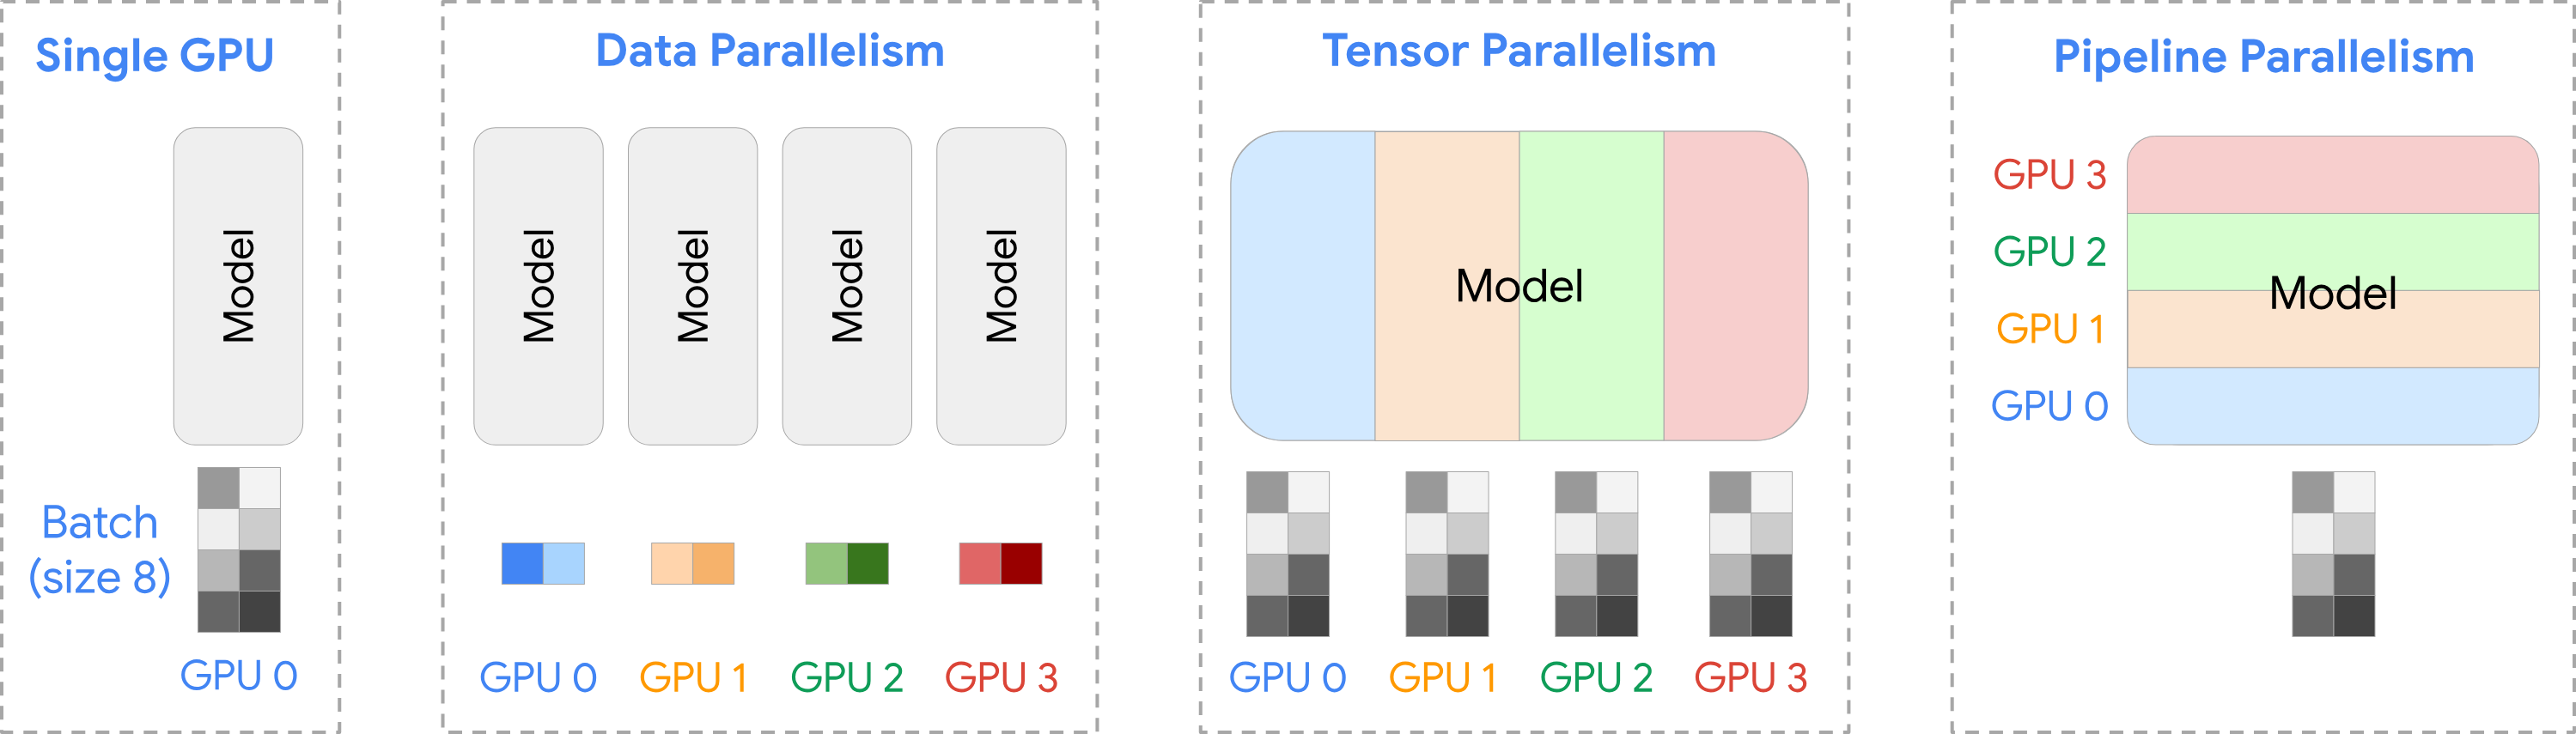
\includegraphics[width=0.75\linewidth]{parallelism classifications.png}
        \label{fig:placeholder}
    \end{figure}

    \item[Message Passing] This model is a communication and synchronization tool between processes. Each processor executes its own program and works on its own private data. To collaborate on the same problem, they communicate by explicitly sending messages to one another. This architecture is derived from distributed computing (clusters). The most representative library for this model is the Message Passing Interface (MPI).

    \begin{figure}[h]
        \centering
        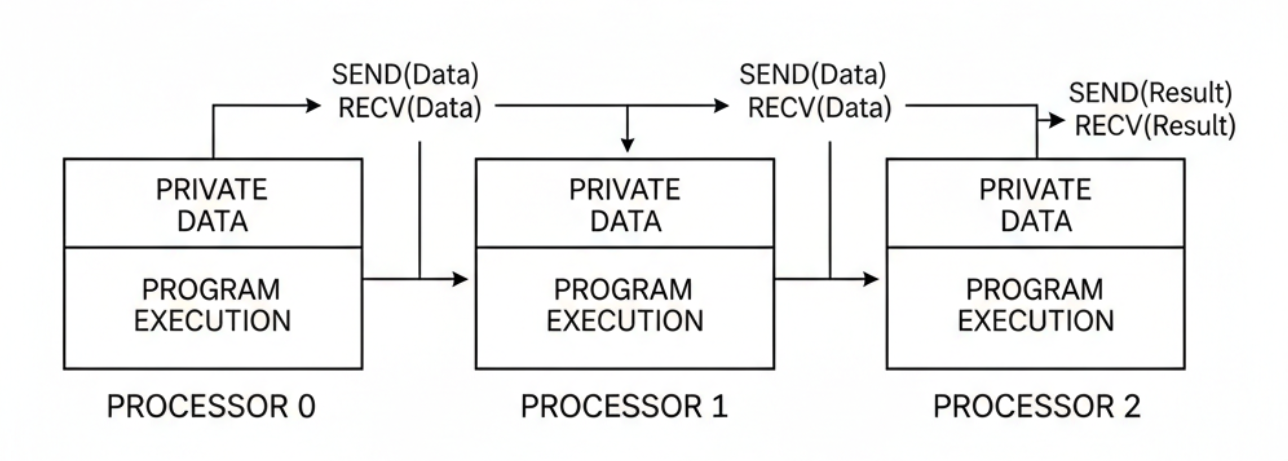
\includegraphics[width=0.75\linewidth]{message passing.png}
        \label{fig:placeholder}
    \end{figure}

    \item[Bit-Level Parallelism] This refers to the mechanism of increasing the processor's word size (the chain of bits it can process at once). Migrating from 32-bit to 64-bit systems, for example, allows the processor to handle more data with a single instruction, thereby reducing the total number of instructions required for certain operations.
    
    \item[Instruction-Level Parallelism (ILP)] This model is based on modifying the order of a program's instructions to group them for parallel execution without altering the final result. Modern processors implement ILP through hardware structures called \textbf{pipelines}, which segment the execution of an instruction into multiple stages (e.g., fetch, decode, execute, write-back). This allows different instructions to be in different stages of execution simultaneously.

\end{description}

\paragraph{Analogy for Pipelining: A Sequential vs. Pipelined Laundry}
Consider laundry as the data and washing, drying, and folding as the operations.
\begin{itemize}
    \item \textbf{Sequentially:} One thread handles one load of laundry from start to finish before beginning the next. If each of the three stages takes one hour, three loads take $3 \times 3 = 9$ hours.
    \item \textbf{As a Pipeline:} As soon as the first load moves from the washer to the dryer, the second load can begin washing. The three stages work in parallel on different loads. The first load still takes 3 hours, but the second finishes 1 hour later, and the third 1 hour after that. Total time for three loads is $3+1+1=5$ hours.
\end{itemize}

\section{Tools for Parallel Programming}
\label{sec:parallel_programming_tools}
The automatic parallelization of a sequential program remains a largely unsolved problem in computer science. Therefore, programmers must use explicit tools to develop parallel software.

\subsection{Languages, APIs, and Frameworks}
\begin{description}
    \item[Languages] Foundational languages like C/C++, Java, and Python provide libraries and constructs for parallel programming.
    \item[APIs (Application Programming Interfaces)] An API is a set of tools and protocols that allows a developer to make requests to another application or system. It may be composed of several libraries. OpenMP and MPI are key examples.
    \item[Libraries] A library is a collection of pre-compiled functions, routines, or reusable code components.
    \item[Frameworks] A framework is a generic, pre-built structure that provides a basic architecture for developers to implement software upon, making application creation more efficient. Hadoop is a well-known example.
\end{description}

\subsection{Levels of Parallel Programming}
\begin{description}
    \item[Level 1 (Abstraction)] In this model, the complexity of parallelism is entirely managed at the hardware level. It demands minimal programming effort, as the parallelism is limited to what the hardware introduces automatically (e.g., pipelining and Simultaneous Multithreading (SMT)).
    \item[Level 2 (Programming)] This is the most powerful level, emphasizing programmer control over the hardware through libraries and tools such as MPI, CUDA, POSIX Threads (pthreads), and OpenMP.
\end{description}

\subsection{Overview of Key APIs: OpenMP and OpenMPI}

\subsubsection{OpenMP (Open Multi-Processing)}
OpenMP is an API standard for constructing parallel programs in the \textbf{shared-memory} model. It was created to facilitate portable, high-level parallel programming. Before OpenMP, programmers had to use lower-level operating system mechanisms or the pthreads library. OpenMP typically uses compiler directives (pragmas) to specify parallel regions, loops, and tasks. In this model, OpenMP threads are mapped to physical cores, with a one-to-one mapping often providing the best performance.

\subsubsection{OpenMPI (Open Message Passing Interface)}
OpenMPI is a high-performance implementation of the MPI standard, developed by academia and industry. It is designed for the \textbf{distributed-memory} programming model, although it also functions on shared and hybrid memory architectures. MPI handles processes, provides fault tolerance, and supports heterogeneous networks. Its key strengths are:
\begin{itemize}
    \item \textbf{Standardization:} MPI is the de facto standard on most High-Performance Computing (HPC) systems.
    \item \textbf{Portability:} Code requires virtually no modification when ported to different platforms.
    \item \textbf{Performance:} Vendors can create hardware-optimized implementations.
    \item \textbf{Functionality:} While it has over 430 routines, most programs can be written with a dozen core functions.
\end{itemize}

\section{Concurrency and Parallelism in Python}
\label{sec:python_concurrency}
Python provides modules for both concurrency and parallelism, but its behavior is dominated by a key feature: the Global Interpreter Lock (GIL).

\subsection{The Global Interpreter Lock (GIL)}
The GIL is a mutex that prevents multiple native threads from executing Python bytecode at the exact same time within a single process. This means that even on a multi-core processor, only one thread can be running Python code at any given moment.

\subsection{Multithreading in Python}
Python's `threading` module implements \textbf{concurrency}. A single process spawns multiple threads, and the OS switches between them, creating the illusion of parallel execution. Due to the GIL, Python multithreading does not provide a speedup for CPU-bound tasks.
\begin{itemize}
    \item \textbf{Benefits:} It is excellent for I/O-bound tasks (e.g., network requests, file operations), as the GIL is released while a thread waits for I/O, allowing other threads to run. It simplifies resource sharing as threads operate in the same memory space.
    \item \textbf{Drawbacks:} It offers no performance increase for computationally intensive algorithms. Debugging can be more difficult due to the non-deterministic nature of thread scheduling.
\end{itemize}

\subsection{Multiprocessing in Python}
Python's `multiprocessing` module achieves true \textbf{parallelism}. It works by creating multiple processes instead of threads. Each process gets its own Python interpreter and memory space, so each has its own GIL and they do not block each other.
\begin{itemize}
    \item \textbf{Benefits:} It is the ideal solution for CPU-bound tasks, as it can fully leverage multiple processor cores.
    \item \textbf{Drawbacks:} Processes have a higher configuration cost (more memory and startup time) than threads. Sharing data between processes is more complex and requires explicit inter-process communication (IPC) mechanisms like pipes or queues.
\end{itemize}

\subsection{Multithreading vs. Multiprocessing: A Comparison}
For parallel computation tasks in Python, multiprocessing is required. However, for operations within C-based libraries like NumPy or PIL, the GIL is often released, allowing threads to run in parallel with an active Python thread.

\begin{table}[h!]
    \centering
    \caption{Comparison of Multithreading and Multiprocessing in Python.}
    \label{tab:threading_vs_multiprocessing}
    \begin{tabular}{|l|p{0.4\textwidth}|p{0.4\textwidth}|}
        \hline
        \textbf{Characteristic} & \textbf{Multithreading (`threading`)} & \textbf{Multiprocessing (`multiprocessing`)} \\
        \hline
        \textbf{Paradigm} & Implements Concurrency & Implements Parallelism \\
        \hline
        \textbf{Parallel Computation} & Not supported due to the GIL & Supported \\
        \hline
        \textbf{Execution Units} & Multiple threads are generated by a single process. & Multiple processes run on multiple cores, each with its own threads. \\
        \hline
        \textbf{Memory} & Shared memory access. & Separate, isolated memory space per process. \\
        \hline
        \textbf{Setup Cost} & Low & High \\
        \hline
        \textbf{Primary Use Case} & I/O-bound tasks, responsive GUIs. & Computationally intensive tasks. \\
        \hline
    \end{tabular}
\end{table}

\subsubsection{The Von Neumann Bottleneck and the Harvard Architecture}
\label{Neumann_Bottleneck}
The most cited consequence of this design is the \textbf{Von Neumann bottleneck}. The root cause of this limitation is the \textbf{shared bus} connecting the CPU to memory, which must be used for both fetching instructions and transferring data. Since these two fundamental operations are constant and cannot occur at the same time, the bus becomes a point of congestion that limits the maximum speed of the system, regardless of how fast the processor is.

As a solution to this problem, the \textbf{Harvard Architecture} was developed. Its defining characteristic is the use of physically separate memories and buses for instructions and data. This allows the CPU to read an instruction and access data simultaneously, eliminating the bottleneck and significantly improving performance. Although the Von Neumann architecture dominates in general-purpose computers, the Harvard architecture is extremely common in systems where performance is critical, such as in microcontrollers and Digital Signal Processors (DSPs).

\chapter{The Sequential Programming Paradigm}
\label{chap:sequential_paradigm}

Before exploring the complexities and capabilities of concurrent systems, it is essential to first establish a firm understanding of the traditional model upon which they are built: the \textbf{sequential programming paradigm}. This chapter details the historical context, defining characteristics, and fundamental structure of sequential processing, concluding with an analysis of its advantages and inherent limitations in the context of modern computing architectures.

\section{Background and Characteristics}
\label{sec:sequential_background}

The principles of sequential programming were formalized through the rise of structured programming, a movement that sought to improve the clarity, quality, and development time of computer programs by using a disciplined, logical approach.

\subsection{Historical Context: The Rise of Structured Programming}
The intellectual foundations for the sequential paradigm as we know it today were laid in the late 1960s and early 1970s.
\begin{itemize}
    \item \textbf{1966:} The history of structured programming arguably begins with the introduction of the \textbf{structured program theorem} by mathematicians Corrado Böhm and Giuseppe Jacopini. They demonstrated that any computable function can be implemented using only three basic control structures: sequence, selection, and iteration.
    \item \textbf{1968:} Dutch computer scientist Edsger W. Dijkstra published his seminal letter, "Go To Statement Considered Harmful." In it, he argued that the indiscriminate use of `goto` statements was a major source of complexity and errors in programs, advocating for the adoption of the high-level control structures identified by Böhm and Jacopini.
    \item \textbf{1970:} The final foundational step was taken by Swiss computer scientist Niklaus Wirth, who developed the programming language \textbf{Pascal}. As one of the first languages designed explicitly to enforce the principles of structured programming, Pascal changed the paradigm of software development and became a cornerstone of computer science education for decades.
\end{itemize}

\subsection{Defining Characteristics}
In serial or sequential processing, a single processor completes one task at a time; subsequent tasks must wait in a queue until the current task is finished. Processors such as the Intel Pentium III and Pentium 4 are classic examples of architectures designed primarily for serial processing. This model is defined by the following characteristics:
\begin{description}
    \item[Deterministic Execution] Sequential processing is a form of computation that executes the same sequence of instructions and, for a given input, will always produce the exact same output. This deterministic behavior presumes no deliberate use of randomness in the algorithm.
    \item[Textual Order of Execution] The textual order of statements in the source code specifies the precise order of their execution. For example, in the statements:
    \begin{verbatim}
    a = b + c;
    d = e - a;
    \end{verbatim}
    It is guaranteed that the value of \texttt{a} will be assigned before the value of \texttt{d} is calculated and assigned.
    \item[Non-Overlapping Execution] From the program's perspective, successive statements are executed without any temporal overlap. The execution of one instruction must complete before the execution of the next one begins.
\end{description}

\section{The Structure of a Sequential Program}
A sequential program is one in which actions (instructions) follow one another in a defined sequence. This structure is built from a few fundamental components and governed by the basic control structures.

\subsection{Fundamental Components}
\begin{description}
    \item[Variable and Constant Declaration] This process consists of listing all variables that will be used at the beginning of the algorithm. In addition to assigning a name, the variable's data type must also be specified.
    \begin{verbatim}
    Counter: INTEGER
    Age: INTEGER
    Address: STRING
    Option: CHARACTER
    \end{verbatim}
    
    \item[Assignment] This is the process of passing values or results to a location in memory (a variable). Assignments can be categorized by their function:
    \begin{itemize}
        \item \textbf{Simple:} Assigning a constant value to a variable (e.g., `a = 15`).
        \item \textbf{Counter:} Using a variable to track the number of times a process is performed (e.g., `a = a + 1`).
        \item \textbf{Accumulator:} Using a variable to sum a set of values during a process (e.g., `a = a + b`).
        \item \textbf{Working:} Assigning the result of a complex mathematical operation involving multiple variables (e.g., `a = c + b * 2 / 4`).
    \end{itemize}
    
    \item[Data Output (Writing)] This consists of sending a result or message to an output device, such as a monitor or printer.
    
    \item[Data Input (Reading)] This consists of receiving a value or datum from an input device, such as a keyboard. This data is then stored in a specified variable.
\end{description}

\subsection{Basic Control Structures}
As established by the structured program theorem, any algorithm can be constructed using only three types of control flow:
\begin{description}
    \item[Sequence] This is the default control structure, where two or more operations are executed in the order they appear in the source code.
    \item[Selection (Conditional)] This structure, commonly implemented with an `if-then-else` statement, refers to the selection of one path of execution from two or more possible alternatives based on a boolean condition.
    \item[Iteration (Loop)] This structure, implemented with `while` and `for` statements, allows for the repetition of a statement or block of statements as long as a boolean condition remains true or for a specified number of times (using a counter).
\end{description}

\subsection{A Concrete Example of a Sequential Algorithm}
To illustrate the principles of sequential programming, let us consider a simple yet fundamental algorithm: finding the maximum value within an unordered array of numbers.

\paragraph{Problem Definition}
Given a non-empty array $A$ of $n$ numerical elements, the task is to find the element $A_i$ such that $A_i \ge A_j$ for all $j \in \{0, 1, \dots, n-1\}$.

\paragraph{Sequential Implementation}
The algorithm proceeds by initializing a candidate for the maximum value with the first element of the array. It then iterates through the remaining elements one by one, updating the candidate whenever a larger element is found. This process is deterministic and its execution path is identical for any given input array.

Below are implementations in Python and Java that demonstrate this sequential logic.

\begin{lstlisting}[language=Python, caption={Sequential maximum-finding algorithm in Python}]
def find_max_sequential(data: list) -> float:
    """
    Finds the maximum value in a list of numbers sequentially.
    """
    if not data:
        raise ValueError("Input list cannot be empty")
    
    max_value = data[0]
    for i in range(1, len(data)):
        if data[i] > max_value:
            max_value = data[i]
            
    return max_value

# Example usage:
my_numbers = [3, 41, 12, 9, 74, 15]
maximum = find_max_sequential(my_numbers)
print(f"The maximum value is: {maximum}")
\end{lstlisting}

\begin{lstlisting}[language=Java, caption={Sequential maximum-finding algorithm in Java}]
public class SequentialMaxFinder {
    public static double findMax(double[] data) {
        if (data == null || data.length == 0) {
            throw new IllegalArgumentException("Input array cannot be empty.");
        }

        double maxValue = data[0];
        for (int i = 1; i < data.length; i++) {
            if (data[i] > maxValue) {
                maxValue = data[i];
            }
        }
        return maxValue;
    }

    public static void main(String[] args) {
        double[] myNumbers = {3.0, 41.0, 12.0, 9.0, 74.0, 15.0};
        double maximum = findMax(myNumbers);
        System.out.println("The maximum value is: " + maximum);
    }
}
\end{lstlisting}

\paragraph{Analysis}
This algorithm perfectly embodies the sequential paradigm. The \texttt{for} loop imposes a strict, linear order of execution. The calculation for index $i$ cannot begin until the calculation for index $i-1$ is complete. The algorithm is characterized by a time complexity of $O(n)$, as it requires a single pass through the array, and a space complexity of $O(1)$, as it uses a constant amount of extra memory regardless of the input size.

\section{Advantages and Limitations of the Sequential Paradigm}
While the sequential paradigm has been superseded in high-performance contexts, its simplicity and predictability provide significant advantages for a wide range of applications.

\subsection{Advantages}
\begin{itemize}
    \item \textbf{Simplicity:} Sequential programs are generally easier to write, read, and understand than their concurrent counterparts.
    \item \textbf{Clarity:} The program's structure is clear, as the flow of control follows the textual layout of the code.
    \item \textbf{Reduced Effort in Debugging:} The deterministic nature of sequential execution makes testing and debugging far more straightforward, as bugs are typically reproducible.
    \item \textbf{Lower Maintenance Costs:} The clarity and simplicity of the code reduce the long-term costs associated with software maintenance.
    \item \textbf{Rapid Development:} For many problems, sequential programs are simpler and faster to design and implement.
\end{itemize}

\subsection{Limitations}
\begin{itemize}
    \item \textbf{Monolithic Structure:} The program often exists as a single, large block of code, which can be difficult to manage.
    \item \textbf{Poor Reusability:} For very large programs, reusing sections of sequential code can be impractical.
    \item \textbf{Execution Bottleneck:} Each instruction must wait for the previous one to complete, creating a fundamental performance bottleneck.
    \item \textbf{Inefficient Resource Utilization:} The sequential model does not take advantage of the multiple processor cores available in modern computer architectures.
    \item \textbf{Unsuitability for HPC:} It is not a viable paradigm for High-Performance Computing (HPC), where problems demand the simultaneous use of vast computational resources.
\end{itemize}
These limitations directly motivate the need for the concurrent and parallel programming paradigms, which will be discussed in the subsequent chapter.


\chapter{Introduction to Concurrent Programming}

Concurrent programming is a fundamental paradigm in modern computing. As systems grow in complexity and the demand for performance increases, the ability to manage multiple tasks simultaneously becomes not just an advantage, but a necessity. This chapter explores the essential concepts of concurrency, from its theoretical foundations to its practical implementations, challenges, and benefits.

\section{Fundamentals of Concurrency}

To understand concurrent programming, we must first establish what it is, how it differs from similar concepts like parallelism, and what its inherent characteristics are.

\subsection{Background and Motivation}
For decades, performance improvements in computing were largely driven by increases in single-processor clock speeds, a trend described by Moore's Law. However, around the mid-2000s, engineers encountered fundamental physical limitations known as the "power wall." Increasing clock speeds further led to prohibitive levels of heat dissipation and power consumption. With the end of single-core frequency scaling, the industry shifted its focus to multi-core architectures. In this new landscape, the only way to leverage the increasing number of transistors for greater performance was to embrace parallelism. This paradigm shift made concurrent programming not just a niche for high-performance computing, but a mainstream necessity for all software development.

\subsection{What is Concurrent Programming?}

In essence, concurrent programming is based on the idea that a computation or algorithm can be divided into independent pieces, where the execution order of these pieces is not strictly sequential. Concurrency is, therefore, a property of the algorithm designed to solve a problem, allowing multiple control flows to advance "at the same time."

It is crucial to distinguish \textbf{concurrency} from \textbf{parallelism}.
\begin{itemize}
    \item \textbf{Concurrency} is the management of multiple tasks at once. A concurrent program can run on a single processor, where the operating system alternates the execution of tasks, creating the \textit{illusion} of simultaneity.
    \item \textbf{Parallelism} is the simultaneous execution of multiple tasks. This is only possible when multiple processors are available, allowing each task to run on a different core at the same time.
\end{itemize}

In summary, concurrency is a logical construction of the software, while parallelism is a physical execution dependent on the hardware. A concurrent program will only run in parallel if the underlying hardware allows it.

\subsection{Key Characteristics of Concurrent Systems}

Concurrent systems are defined by a set of characteristics that distinguish them from traditional sequential systems.
\begin{enumerate}
    \item \textbf{Interaction}: The most defining characteristic is that the system's components (processes or threads) interact with each other. The richness and complexity of these systems arise precisely from this interaction, which can manifest as communication by message passing (synchronous or asynchronous) or through the use of shared memory.
    \item \textbf{Non-Transformational}: Unlike a transformational system that follows an input-process-output sequence, the continuous behavior of a concurrent system is critical. The components evolve in parallel with their environment, collaborating to achieve a common goal rather than simply transforming an input into an output.
    \item \textbf{Unbounded Execution}: Many concurrent systems are designed to run indefinitely. Think of the Internet or an operating system; they are systems whose behavior is best modeled as a potentially infinite sequence of events, so limiting their execution time is inappropriate.
\end{enumerate}

\section{Processes and Threads: The Units of Execution}
Concurrency is implemented through two key concepts: processes and threads.

A \textbf{process} is an instance of a program in execution, an active entity to which the operating system allocates a private set of resources, including a memory address space. In a concurrent system, multiple processes can compete for system resources, but they are isolated from one another.

Every process begins its life with a single, primary \textbf{thread of control}. This is the initial path of execution for the process's code. Concurrency within a process is achieved through \textit{multithreading}, which is the act of creating additional threads of control. A \textbf{thread} is the smallest unit of execution that the OS can schedule. A process can contain multiple threads that share its memory and resources, allowing for closer and more efficient collaboration than inter-process communication.

To ensure their independent control, each thread possesses essential properties:
\begin{itemize}
    \item \textbf{A state}: It can be idle, ready, running, or blocked.
    \item \textbf{A context}: It includes the program counter, processor registers, and a memory stack to store its state when not running.
    \item \textbf{Access to resources}: It has access to the memory and shared resources of the process to which it belongs.
\end{itemize}

\subsection{Benefits and Challenges of Threads}
The use of multiple threads offers significant performance benefits. It takes less time to create, terminate, or switch context between threads of the same process than between separate processes. Additionally, by sharing the same memory space, code duplication in the system's memory is avoided.

However, this advantage introduces great complexity. Sequential programs, with a single thread of control, are much easier to implement and debug. Concurrency, by its nature, generates difficult problems to solve.

\section{The Challenge of Synchronization: Race Conditions}
The main difficulty of concurrent programming lies not in dividing tasks, but in managing the interaction between them.

\subsection{The Problem of Nondeterminism}
The execution of a concurrent program is \textbf{nondeterministic}. This means that the result can vary with each execution, as the interleaving of operations from different threads depends on unpredictable factors, such as the CPU time allocation by the operating system. This nondeterminism is the cause of very difficult errors to detect and correct. Preventing incorrect interleavings from corrupting the program's state is the main problem of synchronization.

\subsection{Race Conditions and \textit{Heisenbugs}}
When multiple threads access and modify a shared resource (like a variable or a file), a \textbf{race condition} can occur. This happens when the final outcome of the operation depends on the relative order and timing of the threads. Sometimes the program will work as expected, and other times it will not, leading to sporadic and hard-to-debug failures.

This type of error is colloquially known as a \textit{Heisenbug}: a bug that seems to disappear or change its behavior when one tries to observe or debug it. The reason is that the act of debugging alters the timing of the threads, hiding the race condition. For this reason, it is fundamental to avoid race conditions through careful design and not through reactive debugging.

\section{Basic Synchronization Mechanisms}
To control nondeterminism and avoid race conditions, processes and threads must synchronize their actions.

\subsection{Communication and Synchronization}
Communication between processes is fundamentally based on two models: the use of \textbf{shared variables} or \textbf{message passing}. When shared memory is used, access to the variables must be done in a synchronized manner to ensure data consistency.

To implement synchronization, building blocks called \textbf{primitives} are used. These are the simplest operations available in a language, such as \texttt{seek(x)}, \texttt{read()}, or \texttt{write(v)} for a shared disk. With these primitives, higher-level mechanisms like mutexes and barriers are built.

Every synchronization event consists of three components:
\begin{enumerate}
    \item \textbf{Acquisition method}: A thread attempts to obtain the right to synchronize (e.g., enter a critical section).
    \item \textbf{Waiting algorithm}: If the right is not available, the thread must wait.
    \item \textbf{Release method}: The thread that holds the right releases it, allowing another to proceed.
\end{enumerate}

\subsection{Waiting Algorithms: Busy-Waiting vs. Blocking}
When a process must wait, there are two main strategies:
\begin{enumerate}
    \item \textbf{Busy-Waiting}: The process executes in a loop, repeatedly checking the value of a shared variable until it changes, indicating that it can continue. Although simple, this method is very inefficient as it consumes CPU time without doing useful work. It is only recommended for very short waiting periods.
    \item \textbf{Blocking}: The process is suspended, notifying the operating system that it is waiting for a specific event. The operating system will not assign it CPU time until another process "wakes it up" after releasing the resource. This method is much more efficient for long waiting periods, as it frees up the processor for other tasks to run.
\end{enumerate}

\section{Mutual Exclusion and Critical Sections}
The most fundamental mechanism to prevent race conditions is mutual exclusion, applied to critical sections of code.

\subsection{The Critical Section}
A \textbf{critical section} is a portion of code that accesses shared resources and that must not be executed by more than one process or thread at a time. If a process is executing its critical section, no other process can enter a critical section that accesses the same resources.

\subsection{Mutual Exclusion (Mutex)}
The problem of \textbf{mutual exclusion} consists of designing a protocol that guarantees that only one process at a time can execute the code of its critical section. This protocol is generally implemented with two operations: \texttt{acquire} before entering the critical section, and \texttt{release} upon exiting. An object that implements this behavior is known as a \textbf{mutex} or a \textbf{lock}.

\subsection{Safety and Liveness Properties}
A correct concurrent solution must satisfy two types of properties:
\begin{enumerate}
    \item \textbf{Safety Properties}: They ensure that "nothing bad happens." The main safety property is mutual exclusion itself: that two processes are never simultaneously in their critical sections.
    \item \textbf{Liveness Properties}: They ensure that "something good eventually happens." They guarantee that the program makes progress. The most important are:
    \begin{itemize}
        \item \textbf{Deadlock-freedom}: Guarantees that if a process tries to enter the critical section, eventually some process will succeed. A deadlock occurs when two or more processes wait for each other in an endless cycle.
        \item \textbf{Starvation-freedom}: A stronger property that guarantees that if a process tries to enter the critical section, \textit{that particular process} will eventually succeed. Starvation occurs when a scheduler indefinitely prevents a ready-to-progress process from being chosen.
    \end{itemize}
\end{enumerate}

\subsection{Necessary Conditions for Deadlock}
A deadlock does not occur by chance. For a system to enter a deadlock state, four conditions, known as the \textbf{Coffman conditions}, must hold simultaneously:
\begin{enumerate}
    \item \textbf{Mutual Exclusion:} At least one resource must be held in a non-shareable mode. That is, only one process at a time can use the resource.
    \item \textbf{Hold and Wait:} A process must be holding at least one resource while waiting to acquire additional resources held by other processes.
    \item \textbf{No Preemption:} Resources cannot be preempted; that is, a resource can be released only voluntarily by the process holding it, after that process has completed its task.
    \item \textbf{Circular Wait:} There must exist a set of waiting processes $\{P_0, P_1, \dots, P_n\}$ such that $P_0$ is waiting for a resource that is held by $P_1$, $P_1$ is waiting for a resource that is held by $P_2$, ..., and $P_n$ is waiting for a resource that is held by $P_0$.
\end{enumerate}
Deadlock prevention or detection focuses on breaking at least one of these four conditions.

\subsection{Solutions for Mutual Exclusion}
There are various strategies to implement mutual exclusion:
\begin{itemize}
    \item \textbf{Software solutions}: Algorithms like Dekker's or Peterson's that use only shared variables. They are of great theoretical value but are complex and prone to errors.
    \item \textbf{Hardware solutions}: Special machine instructions that perform operations like "read and write" atomically, ensuring they cannot be interrupted.
    \item \textbf{Solutions with operating system support}: Higher-level mechanisms like \textbf{semaphores} and \textbf{monitors}, which greatly simplify the programmer's task.
\end{itemize}

\section*{*Advanced Synchronization Mechanisms}
Beyond the basic mutual exclusion provided by mutexes, there are higher-level synchronization primitives that allow for the coordination of more complex interactions between threads.

\subsection*{*Semaphores}
A \textbf{semaphore} is a generalization of a mutex. It is an integer counter that supports two atomic operations: \texttt{wait()} (or \texttt{P}) and \texttt{signal()} (or \texttt{V}).
\begin{itemize}
    \item \texttt{wait()}: Decrements the semaphore's counter. If the counter becomes negative, the process blocks.
    \item \texttt{signal()}: Increments the counter. If there are any processes blocked waiting, one of them is woken up.
\end{itemize}
A semaphore initialized to 1 behaves exactly like a mutex. However, if initialized to a value $N > 1$, it allows up to $N$ threads to access a resource concurrently. This is useful for managing a finite pool of resources, such as a set of database connections.

\subsection*{*Condition Variables}
A \textbf{condition variable} is a synchronization object that allows threads to wait until a specific condition becomes true. They are always used in conjunction with a mutex. A thread acquires the mutex, checks the condition, and if it is not met, it calls \texttt{wait()} on the condition variable. This operation atomically releases the mutex and suspends the thread. Another thread, after changing the state, can call \texttt{signal()} or \texttt{notify()} on the same condition variable to wake up one of the waiting threads, which will then attempt to reacquire the mutex and re-check the condition. They are the fundamental tool for building efficient (non-busy-waiting) solutions to problems like the Producer-Consumer problem.

\section{Thread Implementation in Java}
The Java platform provides a rich, built-in model for concurrent programming, centered on the \texttt{java.lang.Thread} class. There are two primary methodologies for creating a new thread of execution.

\subsection{Extending the \texttt{Thread} Class}
The first approach is to define a new class that inherits directly from \texttt{Thread} and overrides its \texttt{run()} method. The logic to be executed by the new thread is placed within this \texttt{run()} method.

\begin{lstlisting}[language=Java, caption={Creating a thread by extending the Thread class}]
class MyThread extends Thread {
    private String threadName;

    MyThread(String name) {
        this.threadName = name;
    }

    @Override
    public void run() {
        System.out.println("Executing thread: " + threadName);
        try {
            // Simulate some work
            Thread.sleep(1000);
        } catch (InterruptedException e) {
            System.out.println("Thread " + threadName + " interrupted.");
        }
        System.out.println("Thread " + threadName + " finished.");
    }
}

public class ThreadExample {
    public static void main(String[] args) {
        MyThread thread1 = new MyThread("Alpha");
        thread1.start(); // Invokes the run() method in a new thread

        MyThread thread2 = new MyTread("Beta");
        thread2.start();
    }
}
\end{lstlisting}

While straightforward, this method is often less desirable because Java does not support multiple inheritance. If a class must extend another superclass, it cannot also extend \texttt{Thread}.

\subsection{Implementing the \texttt{Runnable} Interface}
The preferred and more flexible approach is to implement the \texttt{java.lang.Runnable} interface. This functional interface requires the implementation of a single method, \texttt{run()}. An object of this class can then be passed to the constructor of a \texttt{Thread} object.

\begin{lstlisting}[language=Java, caption={Creating a thread by implementing the Runnable interface}]
class MyRunnable implements Runnable {
    private String taskName;

    MyRunnable(String name) {
        this.taskName = name;
    }

    @Override
    public void run() {
        System.out.println("Running task: " + taskName);
        // Task logic goes here
    }
}

public class RunnableExample {
    public static void main(String[] args) {
        Thread thread1 = new Thread(new MyRunnable("Task-A"));
        thread1.start();

        // Using a lambda expression for conciseness (Java 8+)
        Thread thread2 = new Thread(() -> {
            System.out.println("Running task: Task-B (from lambda)");
        });
        thread2.start();
    }
}
\end{lstlisting}

\paragraph{Thread Lifecycle and Coordination}
It is critical to distinguish between the \texttt{start()} and \texttt{run()} methods. Invoking \texttt{start()} requests the Java Virtual Machine (JVM) to create a new thread and schedule it for execution, which in turn calls the \texttt{run()} method. Calling \texttt{run()} directly does not create a new thread; it simply executes the method sequentially within the calling thread's context.

To coordinate the completion of threads, the \texttt{join()} method is used. When \texttt{threadA.join()} is called from \texttt{threadB}, \texttt{threadB} will block until \texttt{threadA} has completed its execution. This is a fundamental mechanism for ensuring results from concurrent tasks are available before proceeding.

\section{The Producer-Consumer Problem: A Java Implementation}
The Producer-Consumer problem is a canonical concurrency paradigm used to decouple processes that produce work from processes that consume it. A correct, efficient solution requires careful synchronization to manage the shared buffer and prevent race conditions, deadlocks, and busy-waiting. Below is a robust implementation in Java using \texttt{ReentrantLock} and \texttt{Condition} variables.

\subsection{The Shared Buffer}
The core of the solution is a thread-safe buffer that encapsulates the shared data and all synchronization logic.

\begin{lstlisting}[language=Java, caption={Thread-safe shared buffer for Producer-Consumer}]
import java.util.LinkedList;
import java.util.Queue;
import java.util.concurrent.locks.Condition;
import java.util.concurrent.locks.Lock;
import java.util.concurrent.locks.ReentrantLock;

public class SharedBuffer<T> {
    private final Queue<T> buffer;
    private final int capacity;
    private final Lock lock = new ReentrantLock();
    private final Condition notFull = lock.newCondition();
    private final Condition notEmpty = lock.newCondition();

    public SharedBuffer(int capacity) {
        this.buffer = new LinkedList<>();
        this.capacity = capacity;
    }

    public void put(T item) throws InterruptedException {
        lock.lock();
        try {
            // Use while to guard against spurious wakeups
            while (buffer.size() == capacity) {
                System.out.println("Buffer is full, producer is waiting...");
                notFull.await();
            }
            buffer.add(item);
            System.out.println("Produced: " + item);
            // Signal to a potentially waiting consumer
            notEmpty.signal();
        } finally {
            lock.unlock(); // Ensure lock is always released
        }
    }

    public T get() throws InterruptedException {
        lock.lock();
        try {
            while (buffer.isEmpty()) {
                System.out.println("Buffer is empty, consumer is waiting...");
                notEmpty.await();
            }
            T item = buffer.poll();
            System.out.println("Consumed: " + item);
            // Signal to a potentially waiting producer
            notFull.signal();
            return item;
        } finally {
            lock.unlock();
        }
    }
}
\end{lstlisting}

\subsection{The Producer and Consumer Runnables}
The producer and consumer logic is implemented as \texttt{Runnable} tasks that interact with the shared buffer.

\begin{lstlisting}[language=Java, caption={Producer and Consumer tasks}]
class Producer implements Runnable {
    private final SharedBuffer<Integer> buffer;
    Producer(SharedBuffer<Integer> buffer) { this.buffer = buffer; }
    public void run() {
        for (int i = 0; i < 10; i++) {
            try {
                buffer.put(i);
                Thread.sleep((long)(Math.random() * 100));
            } catch (InterruptedException e) { Thread.currentThread().interrupt(); }
        }
    }
}

class Consumer implements Runnable {
    private final SharedBuffer<Integer> buffer;
    Consumer(SharedBuffer<Integer> buffer) { this.buffer = buffer; }
    public void run() {
        for (int i = 0; i < 10; i++) {
            try {
                buffer.get();
                Thread.sleep((long)(Math.random() * 200));
            } catch (InterruptedException e) { Thread.currentThread().interrupt(); }
        }
    }
}
\end{lstlisting}

\subsection{Driver Program}
The main program initializes the shared buffer and launches the producer and consumer threads.

\begin{lstlisting}[language=Java, caption={Main driver for the Producer-Consumer simulation}]
public class ProducerConsumerDriver {
    public static void main(String[] args) {
        SharedBuffer<Integer> buffer = new SharedBuffer<>(5);
        Thread producerThread = new Thread(new Producer(buffer));
        Thread consumerThread = new Thread(new Consumer(buffer));

        producerThread.start();
        consumerThread.start();
    }
}
\end{lstlisting}

\paragraph{Analysis of the Solution}
This implementation demonstrates several critical concepts for professional concurrent programming. The use of a \texttt{while} loop for the condition check within the \texttt{put} and \texttt{get} methods is mandatory to handle \textit{spurious wakeups}, where a thread can wake from \texttt{await()} without having been signaled. The \texttt{finally} block guarantees that the lock is released, preventing deadlocks even if an exception occurs. The two separate \texttt{Condition} objects, \texttt{notFull} and \texttt{notEmpty}, create a more efficient system than a single condition, as a producer's signal is guaranteed to wake a consumer and vice-versa, avoiding unnecessary context switches.

\section{Concurrent Programming in Python}
Python offers robust tools for concurrent programming through its standard modules.

\subsection{The \texttt{threading} Module}
This module allows for thread-based concurrency. The main class is \texttt{threading.Thread}. To create and run a new thread, the following steps are followed:
\begin{enumerate}
    \item An instance of \texttt{Thread} is created, specifying the function to be executed in the \texttt{target} argument and its parameters in \texttt{args}.
    \item The \texttt{start()} method of the object is invoked. This executes the \texttt{target} function in a new thread of control.
    \item The thread is considered "alive" until its \texttt{target} function finishes.
\end{enumerate}

\begin{lstlisting}[language=Python, caption=Example of thread creation in Python]
import threading
import time

def simple_task(number):
    print(f"Thread {number} has started.")
    time.sleep(2)
    print(f"Thread {number} has finished.")

# Create two threads
thread1 = threading.Thread(target=simple_task, args=(1,))
thread2 = threading.Thread(target=simple_task, args=(2,))

# Start the threads
thread1.start()
thread2.start()

print("The threads have been started from the main program.")

# Wait for the threads to finish
thread1.join()
thread2.join()

print("All threads have finished.")
\end{lstlisting}

\subsection{Lock Objects (\texttt{Lock})}
To implement mutual exclusion in Python, \texttt{Lock} objects are used, the lowest-level synchronization primitive. A \texttt{Lock} can be in two states: "unlocked" or "locked."
\begin{itemize}
    \item \texttt{acquire()}: If the lock is unlocked, it locks it and returns immediately. If it is locked, it blocks the thread until it is released by another.
    \item \texttt{release()}: Changes the lock's state from locked to unlocked. It should only be called from the locked state.
\end{itemize}

\begin{lstlisting}[language=Python, caption=Using a Lock for mutual exclusion]
import threading

balance = 0
lock = threading.Lock()

def deposit(amount):
    global balance
    for _ in range(amount):
        lock.acquire() # Acquire the lock before the critical section
        balance += 1
        lock.release() # Release the lock after the critical section

# ... (code to create and run threads that call deposit)
\end{lstlisting}

\subsection{The \texttt{multiprocessing} Module}
Unlike \texttt{threading}, the \texttt{multiprocessing} module uses processes instead of threads. This allows it to bypass Python's "Global Interpreter Lock" (GIL) and take full advantage of multiple processors to achieve real parallelism. Its interface is very similar to that of \texttt{threading}, with a \texttt{Process} class that mimics the methods of \texttt{Thread}.

\section{A Classic Problem: Producer-Consumer}
The producer-consumer problem is a classic paradigm in concurrent programming.

\subsection{Problem Description}
There are two types of processes: \textbf{producers}, which generate data, and \textbf{consumers}, which use it. The challenge is to synchronize them to ensure that each piece of data produced is consumed exactly once, and that consumers do not try to consume data that has not yet been produced.

\subsection{Solution with a Shared Buffer and Condition Variables}
The standard, efficient solution uses a fixed-size \textbf{circular buffer} as a shared storage space. To manage access and coordination safely and without busy-waiting, three synchronization components are required:
\begin{itemize}
    \item \textbf{A Mutex (Lock):} To guarantee \textbf{mutual exclusion}. Any access to the buffer (to add or remove items, or to check its state) must be done within a critical section protected by this mutex.
    \item \textbf{A Condition Variable (\texttt{not\_full}):} For the producer to wait efficiently when the buffer is full. If a producer acquires the lock and sees that there is no space, it calls \texttt{wait()} on this variable, releasing the mutex and becoming suspended.
    \item \textbf{A Condition Variable (\texttt{not\_empty}):} For the consumer to wait efficiently when the buffer is empty. If a consumer acquires the lock and finds no items, it calls \texttt{wait()} on this variable, releasing the mutex and becoming suspended.
\end{itemize}
When a consumer removes an item, it frees up space, so it calls \texttt{signal()} on the \texttt{not\_full} variable to wake up a potentially waiting producer. Analogously, when a producer adds an item, it calls \texttt{signal()} on the \texttt{not\_empty} variable to wake up a consumer. This model is fundamental and is found in countless real-world applications, such as task queues or data streaming.

\section{Balance: Advantages and Limitations}
Finally, it is important to weigh the benefits and drawbacks of adopting a concurrent approach in software development.

\subsection{Advantages of Concurrent Programming}
\begin{itemize}
    \item \textbf{Performance}: It allows solving problems in a reasonable time that would be infeasible on a single CPU, achieving significant speedup.
    \item \textbf{Scalability}: It facilitates the division of tasks into independent parts, which allows for great expansion and scalability as hardware resources increase.
    \item \textbf{Capability}: It makes it possible to tackle problems of a greater order and complexity that could not be handled by a sequential system.
\end{itemize}

\subsection{Limitations and Challenges}
\begin{itemize}
    \item \textbf{Complexity}: The main disadvantage is the inherent difficulty in writing, debugging, and maintaining concurrent programs. Achieving correct synchronization is a complex task prone to subtle errors.
    \item \textbf{Costs}: The development and maintenance of concurrent systems can have higher costs. Additionally, the intensive use of multiple processors can increase energy consumption.
    \item \textbf{Overhead}: Communication and synchronization between tasks introduce delays and consume resources, which can, in some cases, nullify performance gains.
\end{itemize}

\end{document}